% ----------------------------------------------------------
\chapter{Identificação de interferências e falhas no monitoramento de baixo custo}\label{cap:field-monit-results}
% ----------------------------------------------------------

Utilizando uma das placas CLEAN Arduino Mega descritas no Capítulo \ref{cap:clean-initiative}, foi desenvolvido um equipamento de baixo custo para monitoramento dos poluentes \acrshort{co}, \acrshort{no2}, \acrshort{so2}, \acrshort{o3} e \acrshort{mp10}. Para medição desses poluentes o instrumento conta com a seguinte relação de sensores:

\begin{itemize}
    \item Um sensor eletroquímico do fabricante Alphasense modelo CO-B4 para medição da concentração de \acrshort{co}
    \item Dois sensores eletroquímicos do fabricante Alphasense modelo SO2-B4 para medição da concentração de \acrshort{so2}
    \item Um sensor eletroquímico do fabricante Alphasense modelo NO2-B43F para medição da concentração de \acrshort{no2}
    \item Dois sensores eletroquímicos do fabricante Alphasense modelo OX-B431 para medição da concentração de \acrshort{o3}
    \item Um sensor ótico do fabricante Alphasense modelo OPC-N3 para medição da concentração de \acrshort{mp10} e \acrshort{mp25}
    \item Um sensor de temperatura para medição da temperatura dentro da câmara de medição dos gases.
\end{itemize}

O instrumento foi instalado junto a uma estação de referência no município de Tubarão por um período de 5 meses, desde 21/11/2022 até 21/04/2023. O objetivo da instalação foi testar o dispositivo em campo, numa aplicação real e adquirir leituras de concentração dos sensores para posteriormente de calibrar o instrumento com os dados da estação de referência.

% ----------------------------------------------------------
\section{Correção das leituras por co-localização}
% ----------------------------------------------------------

A co-localização consiste em instalar o equipamento de baixo custo junto a uma estação de monitoramento de referência para fins de validação e correção. Para cobrir as diversas condições atmosféricas, a sazonalidade, e a gama de valores de concentração dos gases de interesse e dos gases interferentes, a literatura recomenda uma duração de três a seis meses para a execução das rotinas de testes e validação \cite{Spinelle2013ProtocolPollution}.

Na aplicação apresentada neste trabalho, o instrumento de baixo custo desenvolvido foi instalado por cinco meses junto a uma estação de referência localizada no bairro Vila Moema, no município de Tubarão - SC. A estação é uma das três que fazem parte atualmente da rede de monitoramento do estado de Santa Catarina, operadas pela Diamante Geração de Energia Ltda. \cite{IMASC24}. O município de Tubarão é vizinho de Capivari de Baixo, onde se encontra o complexo termelétrico Jorge Lacerda, operado também pela Diamante Geração de Energia Ltda. A Figura \ref{fig:stations-map} ilustra a localização geográfica das estações de monitoramento na região de Capivari de Baixo, e Tubarão. Na Tabela relacionam-se os equipamentos presentes na estação Vila Moema onde foi instalado o instrumento de baixo custo desenvolvido.

\begin{figure}[h]
    \centering
    \caption{Mapa das estações de monitoramento em Tubarão e Capivari de Baixo}
    \includegraphics[width=0.9\textwidth]{chapters/3-ANÁLISE DOS DADOS/Figuras/mapa-de-estações.png}
    \label{fig:stations-map}
    \fonte{\cite{IMASC24}}
\end{figure}

\begin{table}[!ht]
    \centering
    \caption{Relação de equipamentos presentes na estação de monitoramento de referência no município de Tubarão - SC}
    \begin{tabular}{l|l|l|l}
        \textbf{Equipamento} & \textbf{Poluentes} & \textbf{Princípio de operação} & \textbf{Fabricante} \\
        \hline
        Monitor APNA-370 & NO, NO2 e NOx & Quimioluminescência & Horiba \\
        Monitor APOA-370 & O3 & Adsorção ultravioleta & Horiba \\
        Monitor APSA-370 & SO2 & Fluorescência ultravioleta & Horiba \\
        Monitor APMA-370 & CO & Modulação cruzada & Horiba \\
         & & infravermelha sem dispersão & \\
        Monitor BAM 1020 & MP2.5, MP10 & Atenuação de raios beta & Met One \\
        \hline
    \end{tabular}
    \label{tab:reference-equipments}
\end{table}

Os dados registrados pelos equipamentos de referência são compilados em relatórios diários onde as leituras de concentração são registradas como médias horárias. Para a validação do equipamento de baixo custo, o Instituto do Meio Ambiente de Santa Catarina disponibilizou os relatórios de concentrações de poluentes no período em questão. O instrumento desenvolvido registra as leituras dos sensores com um período de amostragem de 15 minutos. Os dados adquiridos foram filtrados, pré-processados e re-amostrados em médias horárias antes de efetuar as rotinas de correção das leituras com base nas medições da estação de referência.

% ----------------------------------------------------------
\section{Pré-processamento dos dados}
% ----------------------------------------------------------

A primeira etapa no tratamento das leituras dos sensores de gases foi o pré-processamento dos dados para reduzir ruído, identificar falhas e valores atípicos. Para isso os dados foram etiquetados seguindo alguns pontos dos procedimentos descritos por \textit{AQMesh}, Ottosen e Kumar \cite{Ottosen2019OutlierMeasurements} e o Guia para monitoramento da qualidade do ar o IMA \cite{INSTITUTODEENERGIAEMEIOAMBIENTE2019QualidadeAr}. O pré-processamento foi realizado utilizando a linguagem de programação Python e \textit{Jupyter Notebooks}. A continuação descrevem-se cada uma das fases de pré-processamento aplicadas aos dados dos sensores, sumarizadas graficamente na Figura \ref{fig:preprocessing-flow}.

\begin{figure}[h!]
    \centering
    \caption{Fluxograma das etapas de pré-processamento e as etiquetas de saída em cada uma delas}
    \includegraphics[width=0.75\textwidth]{chapters/3-ANÁLISE DOS DADOS/Figuras/Fluxograma pré-processamento.png}
    \label{fig:preprocessing-flow}
\end{figure}

\begin{enumerate}
    \item Suavização das curvas de dados com uma janela temporal de 1 hora: Primeiramente foi realizada a suavização das séries originais buscando reduzir o impacto de flutuações de curto prazo e realçar padrões de longo prazo, dado que os dados de referência encontram-se em períodos horários.
    \item Remoção do Período de Estabilização: Os primeiros 7 dias da série temporal foram desconsiderados. Essa decisão fundamenta-se na consideração de que nesse período inicial após a instalação o sensor encontra-se num estado de estabilização propenso a flutuações e ajustes. A remoção desses dados iniciais visa mitigar possíveis distorções na análise decorrentes desse período transitório.
    \item Remoção de valores fora de intervalo de medição: Em seguida, foram removidos os valores abaixo da resolução do sensor e acima do valor máximo do sensor. Tal procedimento tem por objetivo eliminar possíveis ruídos, registros muito extremos e falhas no sistema de medição que poderiam comprometer a integridade da série temporal.
    \item Remoção de valores com alterações na linha base: Para a detecção dos pontos em que a linha base das leituras sofreu alterações aplicou-se algoritmo \acrshort{pelt} \cite{Killick2012OptimalCost}. Este método foi aplicado por Ottosen e Kumar \cite{Ottosen2019OutlierMeasurements} para detectar mudanças abruptas na média e/ou na variância das séries temporais de sensores de gases. As leituras que apresentaram alterações na linha base foram desconsiderados já que nesses intervalos a distribuição dos dados mudou, dificultando a análise.
    \item Remoção de outliers por quartis: Consistiu na remoção dos quartis 1\% e 99\% dos dados agrupados por hora. Esse processo foi conduzido após a divisão dos dados em 24 grupos, representando cada hora do dia. Os quartis foram calculados individualmente dentro desses grupos, resultando em uma eliminação robusta de extremos estatísticos que poderiam introduzir viés na análise.
    \item Identificação e remoção de picos e outliers na derivada dos dados: Este passo envolveu a identificação e eliminação de picos na primeira derivada dos dados que excediam o valor máximo encontrado na derivada da série de dados de referência. Essa estratégia visa mitigar efeitos de variações abruptas, frequentemente associadas a falhas no sensor ou interferências externas.
    \item Re-amostragem para período de 1 hora: Este passo consistiu na re-amostragem dos dados para um período de 1 hora. Essa prática foi adotada para comparar e calibrar com os dados de referência que estão em períodos de uma hora.
    \item Remoção de médias com amostras insuficientes: Por fim, foram excluídas as médias de cada hora que não atingiram mais de 75\% de amostras válidas, equivalente a pelo menos 3 amostras por hora. Essa medida visa garantir a robustez estatística das médias horárias, excluindo intervalos com dados insuficientes para uma análise significativa.
\end{enumerate}

Em cada estágio do pré-processamento, os dados eram etiquetados para diferenciar as leituras válidas das que apresentaram algum tipo de anomalia que inviabilizasse seu uso. A seguir são listadas as etiquetas utilizadas para identificar cada amostra; entre parênteses colocasse o nome da etiqueta utilizada dentro do código. O Anexo \ref{anex:preprocessing-notebooks} contêm o código desenvolvido em \textit{Jupyter Notebooks} para executar esta etapa da análise dos dados.

\begin{itemize}
    \item Dados faltantes (\textit{MISSING}): Esta etiqueta representa amostras faltantes na amostragem dos dados.
    \item Estabilização (\textit{STABILIZ}): A estabilização é um período em que um sensor fornece dados não confiáveis por não estar em estado de equilíbrio. Uma vez que o sensor se estabilizar em seu ambiente após ter sido movido recentemente ou após ter sido instalado pela primeira vez, ele fornecerá dados utilizáveis. Este processo leva 2 dias para ser concluído para sensores eletroquímicos, não sendo necessário para o sensor de material particulado modelo OPC de Alphasense (Manual de procedimento de operação padrão AQMesh). Neste trabalho foi utilizado um período de 7 dias para garantir uma maior estabilidade do sensor.
    \item Dados acima do Limite Superior (\textit{GTUL}): Essa etiqueta está relacionada a valores que ultrapassam o limite superior do sensor. As especificações do fabricante ou valores conhecidos do poluente podem ser utilizados para definir esse limite. Por exemplo, o sensor Alphasense CO-B4 tem um limite de 1.000 ppm, equivalente a 1.000.000 ppb. Os valores que ultrapassaram esses limites para cada sensor foram removidos por serem indícios de alguma falha ou mal funcionamento do sistema de medição.
    \item Dados abaixo do Limite Inferior (\textit{LTLL}): Esta etiqueta sugere valores que estão abaixo da resolução do sensor e pode estar relacionada a possíveis valores negativos. A definição desse limite depende das especificações do sensor utilizado. O sistema de medição desenvolvido identifica valores faltantes ou NaN com o valor -9999.99. Por esse motivo, valores abaixo de -1000 ppb nos dados representam estas amostras depois de passar pelo processo de suavização.
    \item Dados com alteração do valor de linha base (\textit{REBASE}): Nas séries temporais dos sensores foram identificados alterações no valor de linha base das leituras. Observou-se também que nesses intervalos de variação da linha base a distribuição dos dados também estava alterada. Por esse motivo, os dados nesses intervalos foram marcados e removidos.
    \item Dados do quartil 99 \% (\textit{GTQTLE99}): Essa etiqueta está relacionada aos valores que se encontram no quartil 99 \% no histograma dos dados. Valores dentro desse intervalo foram etiquetados para remoção.
    \item Dados do quartil 1 \% (\textit{LTQTLE01}): Essa etiqueta está relacionada aos valores que se encontram no quartil 1 \% no histograma dos dados. Valores dentro desse intervalo foram etiquetados para remoção.
    \item Baixo número de amostras (\textit{LOWSAMPLES}): De acordo com o Guia de Monitoramento da Qualidade do Ar (IMA), pelo menos 3/4 das medições de uma hora devem ser válidas para o cálculo da média horária. No sistema desenvolvido, como o período de amostragem foi de 15 minutos, para uma média horária ser considerada válida, ela deve ser calculada por 3 ou 4 pontos.
    \item Transições abruptas nos dados (\textit{BADSPIKE}): Transições muito abruptas na série de dados também foram identificados. Para isso foram calculadas as derivadas das séries temporais e os valores comparados com o valor máximo das derivadas das séries temporais de referência. Valores de derivadas na série de dados acima desse valor máximo foram identificados como transições muito abruptas e etiquetados para remoção.
    \item Dados inválidos de temperatura \textit{INVALID\_ENV}: Aos dados de temperatura também foram aplicadas as etiquetas descritas anteriormente, com exceção de \textit{STABILIZ} e \textit{BADSPIKE}. Os valores de concentração de gás adquiridos no mesmo instante de algum dado inválido de temperatura foram marcados como \textit{INVALID\_ENV} para remoção.    
\end{itemize}

% ----------------------------------------------------------
\section{Análise dos dados de Monóxido de Carbono}
% ----------------------------------------------------------

A metodologia de pre-processamento dos dados descrita acima foi aplicada as leituras obtidas pelo sensor de \acrshort{co}. A Figura \ref{fig:data-co-raw} mostra a série temporal do sensor depois de removidos os valores fora de intervalo. Observa-se que a partir do mês de fevereiro ocorreram seguidas alterações de linha base, detectadas pelo algoritmo \acrshort{pelt}, conforme se ilustra na Figura \ref{fig:data-rebase-co}. No histograma das leituras do sensor em questão (Figura \ref{fig:data-co-raw-hist}) observa-se que as mudanças de linha base alteraram também a distribuição dos dados nesse período. Dado que as mudanças de linha base se mantiveram de forma continuada a partir desse mês, para o restante das análises apenas foram consideradas as leituras anteriores à primeira alteração da linha base do sensor. A Figura \ref{fig:data-co-preproc-hist} mostra o histograma dos dados das leituras prévias às alterações de linha base.

\begin{figure}[h]
    \centering
    \caption{Histograma das leituras do sensor CO-B4}
    \begin{subfigure}{0.4\textwidth}
        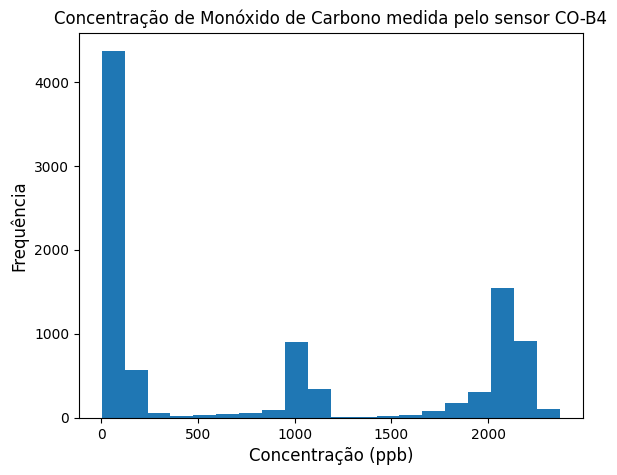
\includegraphics[width=\textwidth]{chapters/3-ANÁLISE DOS DADOS/Figuras/raw-co-b4-hist.png}
        \caption{Histograma prévio à remoção das alterações de linha base}
        \label{fig:data-co-raw-hist}
    \end{subfigure}
    \hfill
    \begin{subfigure}{0.4\textwidth}
        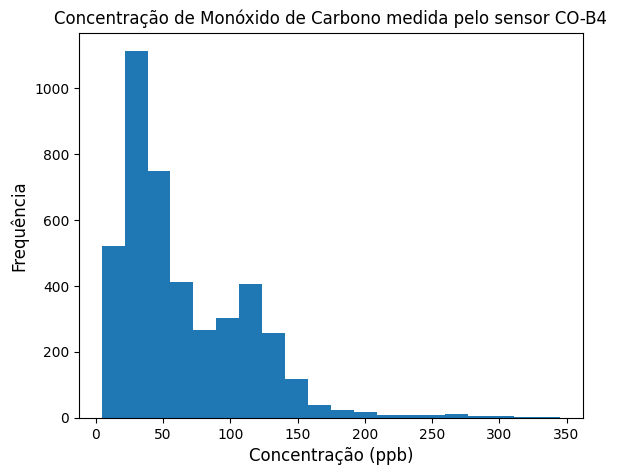
\includegraphics[width=\textwidth]{chapters/3-ANÁLISE DOS DADOS/Figuras/preproc-hist-co-b4.png}
        \caption{Histograma após à remoção das alterações de linha base}
        \label{fig:data-co-preproc-hist}
    \end{subfigure}
    \hfill
    \label{fig:data-co-hist}
\end{figure}

Depois de pré-processadas as leituras do sensor obtiveram-se os resultados ilustrados na Figura \ref{fig:data-co-preproc-15}. A Figura mostra a série de dados pré-processados do sensor CO-B4, juntamente com um gráfico de caixas que representa o comportamento diário das leituras agrupadas por hora do dia. Neste último percebe-se um comportamento periódico nos dados, observando-se maiores valores de amplitude e dispersão durante o período diurno. Ao comparar esse comportamento com os valores de referência percebe-se que a componente diária é mais evidente no sensor CO-B4, indicando uma possível relação com a sazonalidade diária da temperatura.

\begin{figure}[h]
    \centering
    \caption{Série temporal do sensor pré-processada (T = 15 mins) e seu comportamento diário}
    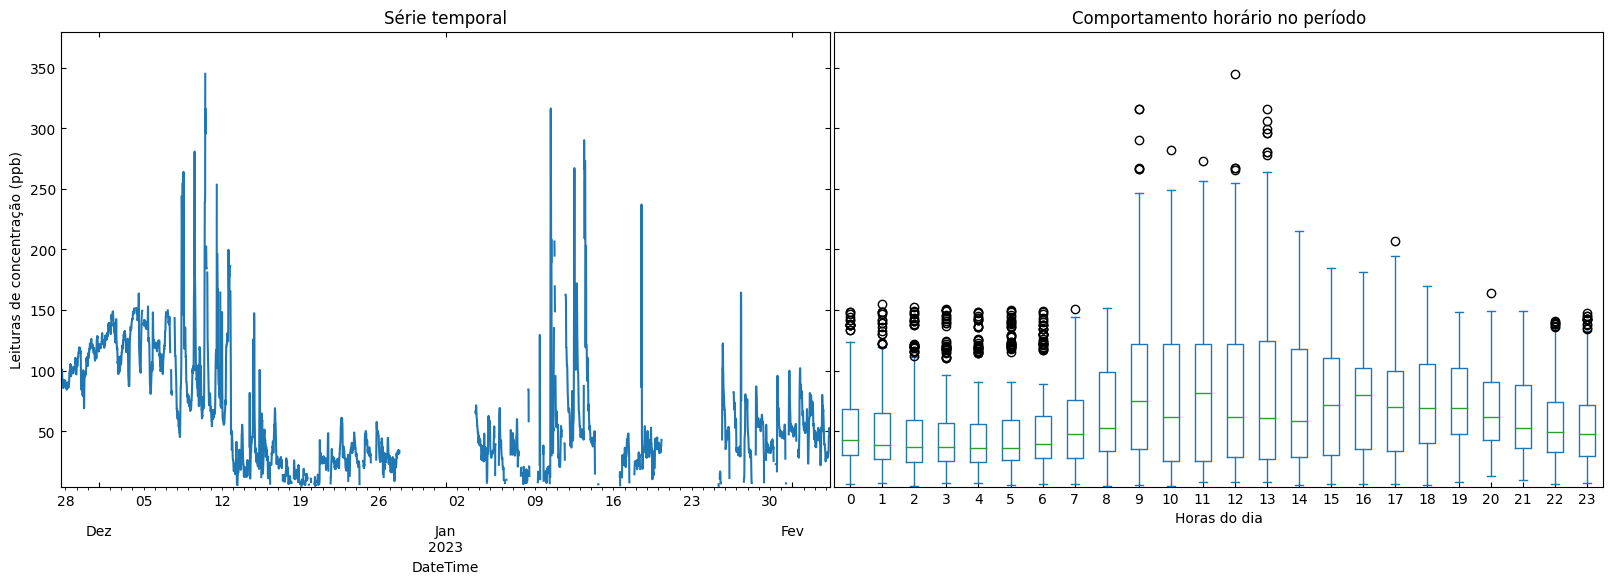
\includegraphics[width=\textwidth]{chapters/3-ANÁLISE DOS DADOS/Figuras/preproc-co-b4.png}
    \label{fig:data-co-preproc-15}
\end{figure}

\begin{figure}[h]
    \centering
    \caption{Série temporal das leituras de concentração de referência (T = 1 H) e seu comportamento diário}
    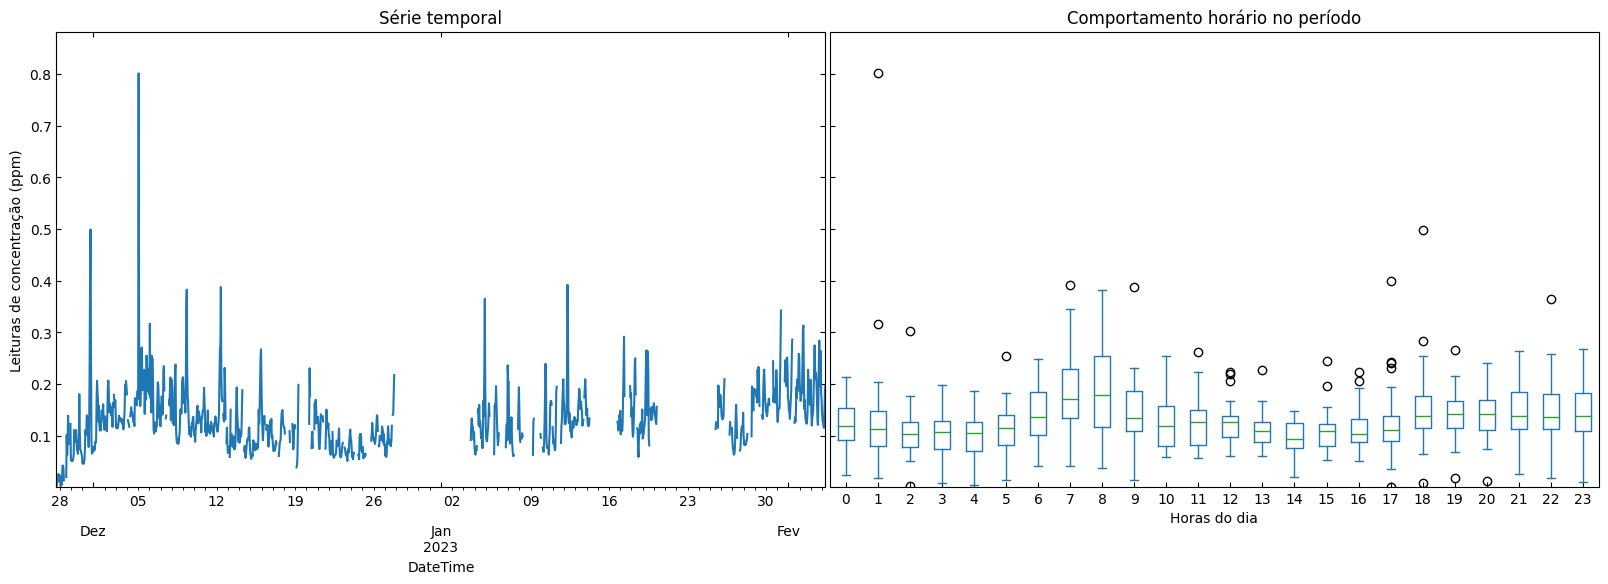
\includegraphics[width=\textwidth]{chapters/3-ANÁLISE DOS DADOS/Figuras/co-reference-series-and-box.png}
    \label{fig:data-co-reference}
\end{figure}

A Figura \ref{fig:data-co-preproc-1HR} mostra a série temporal das leituras do sensor consideradas como válidas, com período de amostragem horário.

\begin{figure}[h]
    \centering
    \caption{Série temporal com T = 1 hr}
    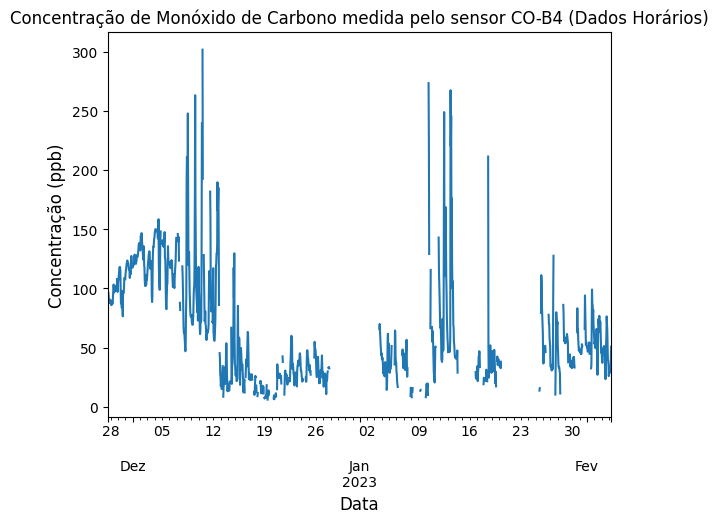
\includegraphics[width=0.5\textwidth]{chapters/3-ANÁLISE DOS DADOS/Figuras/preproc-1HR-co-b4.png}
    \label{fig:data-co-preproc-1HR}
\end{figure}

A Tabela \ref{tab:data-contab-co} mostra a contagem dos dados etiquetados para períodos de 15 minutos e de 1 hora. Observa-se que dos 17647 pontos de dados, que representavam as amostras adquiridas com um período de 15 minutos no intervalo de 20/11/2022 até 23/05/2023, 4270 foram aproveitados como dados válidos, o que representa um 24 \% aproximadamente dos dados originais. Ao re-amostrar esses 4270 pontos em dados horários obtiveram-se 1048 amostras horárias de concentração válidas (aproximadamente 64 \% dos dados) para realizar a calibração.

\begin{table}[h]
    \caption{Contabilização das leituras do sensor CO-B4 por etiquetas}
    \centering
    \begin{tabularx}{0.95\textwidth}[h]{
         >{\raggedright\hsize=.475\hsize\arraybackslash}X
         >{\raggedright\hsize=.20\hsize\arraybackslash}X 
         >{\raggedright\hsize=.5\hsize\arraybackslash}X
        | >{\raggedright\hsize=.50\hsize\arraybackslash}X 
         >{\raggedright\hsize=.20\hsize\arraybackslash}X 
         >{\raggedright\hsize=.5\hsize\arraybackslash}X }
        \multicolumn{3}{c|}{Série temporal T = 15 mins} & \multicolumn{3}{c}{Série temporal T = 1 hr} \\
        \hline
        Etiquetas & No. amostras & \% amostras & Etiquetas & No. amostras & \% amostras \\ [0.5ex]
        \hline
        \textit{MISSING} & 5756 & 32.62 \% & \textit{LOWSAMPLES} & 603 & 36.52 \% \\ [0.5ex]
        
        \textit{LTLL} & 1560 & 8.84 \% & \textit{VALID} & 1048 & 63.48 \% \\ [0.5ex]
        
        \textit{GTUL} & 0.0 & 0.0 \% & & & \\ [0.5ex]
        
        \textit{STABILIZING} & 673 & 3.81 \% & & & \\ [0.5ex]
        
        \textit{BADSPIKE} & 3 & 0.02 \% & & & \\ [0.5ex]
        
        \textit{LTQTLE01} & 63 & 0.36 \% & & & \\ [0.5ex]
        
        \textit{GTQTLE99} & 63 & 0.36 \% & & & \\ [0.5ex]
        
        \textit{REBASE} & 5259 & 29.80 \% & & & \\ [0.5ex]
        
        \textit{VALID} & 4270 & 24.20 \% & & & \\ [0.5ex]
        \hline
        TOTAL & 17647 & & TOTAL & 1651 & \\
    \end{tabularx}
    \label{tab:data-contab-co}
\end{table}

\subsection{Dependência com a temperatura}

Investigou-se a existência de correlação entre as leituras do sensor de \acrshort{co} e as variações de temperatura medida no interior da câmara de medição. Para tal, foram empregados os testes estatísticos de correlação de Spearman e Kendall, por serem métodos não paramétricos que exploram a relação monotônica entre variáveis. Os resultados desses testes revelaram coeficientes de correlação significativos. O coeficiente de Spearman calculado foi de 0.52, com um valor de p inferior a 0.05, indicando uma correlação estatisticamente significativa entre as leituras do sensor e a temperatura. De maneira semelhante, o coeficiente de Kendall foi de 0.38, também com p < 0.05, reforçando a presença de uma associação significativa. Ao avaliar a hipótese nula de ausência de correlação, os resultados forneceram evidências robustas para sua rejeição, sugerindo que há uma correlação entre as leituras do sensor de \acrshort{co} e as variações de temperatura. A Figura \ref{fig:data-temp-co-corr} mostra um gráfico de dispersão entre os dados do sensor e a temperatura, ilustrando os resultados de correlação obtidos. 

\begin{figure}[h]
    \centering
    \caption{Relação dos dados de concentração de \acrshort{co} com a temperatura}
    \begin{subfigure}{0.4\textwidth}
        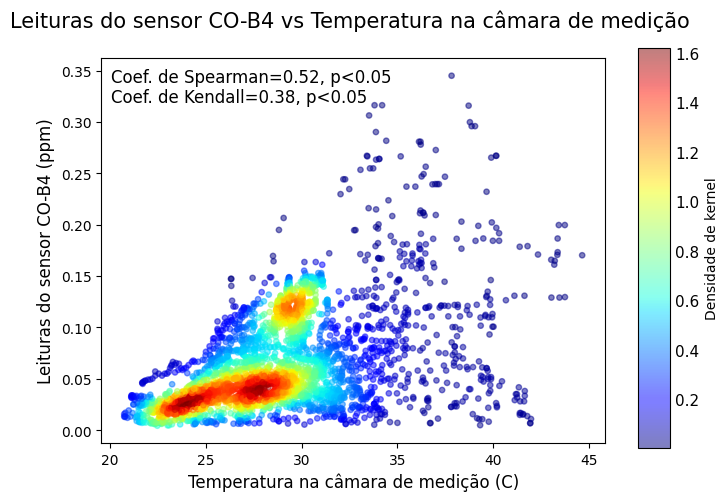
\includegraphics[width=\textwidth]{chapters/3-ANÁLISE DOS DADOS/Figuras/temperature-co-b4.png}
        \caption{Relação entre as leituras do sensor CO-B4 (ppm) e a temperatura (\textdegree C)}
        \label{fig:data-temp-co-corr}
    \end{subfigure}
    \hfill
    \begin{subfigure}{0.4\textwidth}
        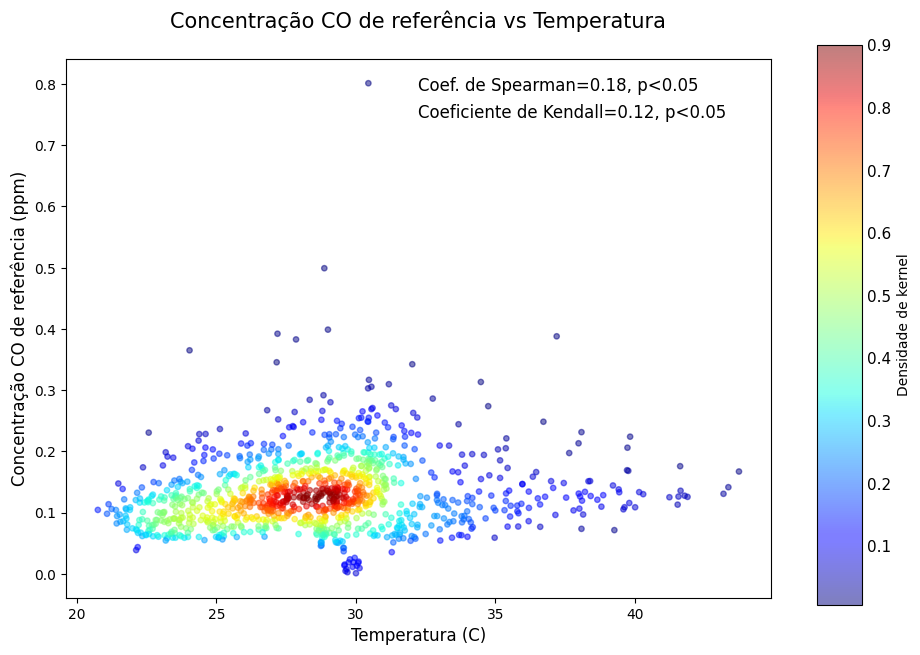
\includegraphics[width=\textwidth]{chapters/3-ANÁLISE DOS DADOS/Figuras/temperature-co-reference.png}
        \caption{Relação entre os valores de concentração de referência (ppm) e a temperatura (\textdegree C)}
        \label{fig:data-temp-co-ref-corr}
    \end{subfigure}
    \hfill
    \label{fig:data-co-temp}
\end{figure}

Os resultados obtidos nos testes estatísticos podem ser corroborados no gráfico de dispersão entre as variáveis. Na Figura \ref{fig:data-temp-co-corr} observam-se dois núcleos principais de dados. O menor deles comporta os valores de concentração entre 0.10 e 0.15 ppm dentro de um intervalo de temperatura de 28 a 30\textdegree C. No segundo núcleo encontram-se valores de concentração entre 0 e 0.06 ppm aproximadamente e de 22 até 30\textdegree C. Neste último grupo de dados é possível apreciar uma clara relação linear entre as leituras do sensor e a temperatura. Ao analisar a relação entre as medições de concentração de referência e a temperatura, também se observa alguma correlação, embora em menor medida, com coeficientes de Spearman e Kendall de 0.18 e 0.12 respectivamente (Figura \ref{fig:data-temp-co-ref-corr}).

\subsection{Calibração das leituras do sensor CO-B4 com as medições de referência}

Nas Figuras \ref{fig:data-co-reference-time-series} e \ref{fig:data-co-reference-corr} apresentam-se as leituras de \acrshort{co} obtidas pelo sensor CO-B4 de Alphasense e a estação de referência. Observa-se que as leituras do sensor CO-B4 em geral subestimaram os valores de concentração de referência. Os testes de Spearman e Kendall revelaram a existência de correlação entre as medições com o sensor de baixo custo e a referência com coeficientes de 0.3 e 0.2 respectivamente.

\begin{figure}[h]
    \centering
    \caption{Séries temporais e gráficos de dispersão das medições de \acrshort{co}}
    \begin{subfigure}{0.44\textwidth}
        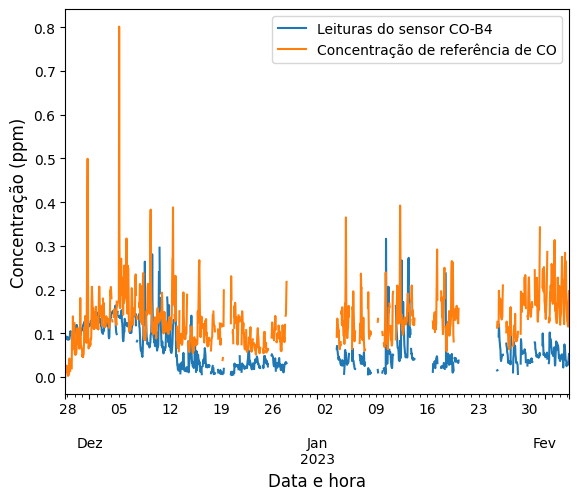
\includegraphics[width=\textwidth]{chapters/3-ANÁLISE DOS DADOS/Figuras/co-b4-reference-time-series.png}
        \caption{Séries temporais das leituras do sensor CO-B4 e a estação de referência}
        \label{fig:data-co-reference-time-series}
    \end{subfigure}
    \hfill
    \begin{subfigure}{0.54\textwidth}
        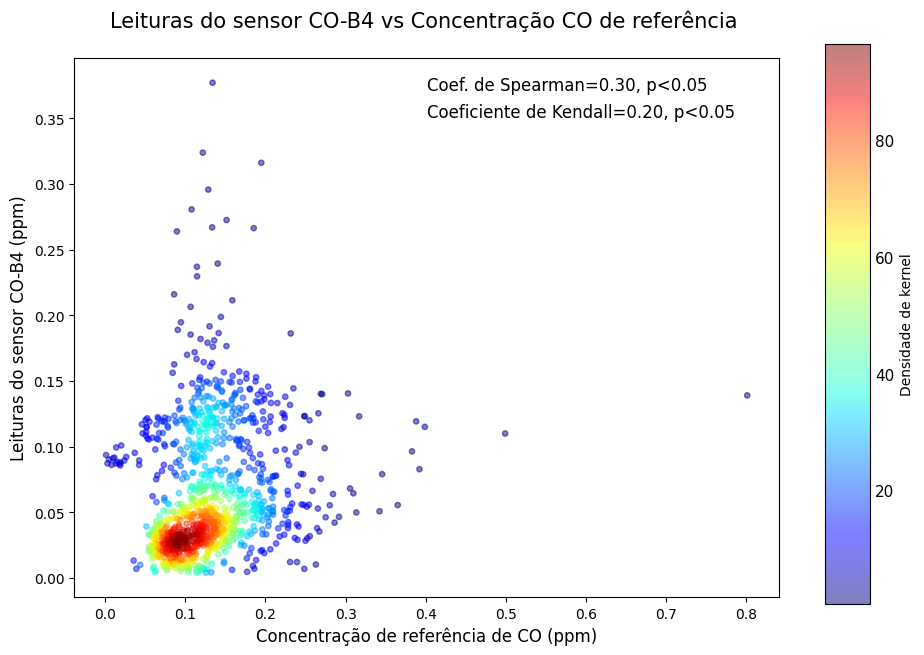
\includegraphics[width=\textwidth]{chapters/3-ANÁLISE DOS DADOS/Figuras/co-b4-reference-correlation.png}
        \caption{Gráfico de dispersão das leituras do sensor CO-B4 e a estação de referência}
        \label{fig:data-co-reference-corr}
    \end{subfigure}
    \fonte{Desenvolvido pelo autor (2023)}
\end{figure}

\begin{table}[h!]
    \caption{Resultados da calibração do sensor CO-B4}
    \centering
    \begin{tabularx}{0.95\textwidth}[h!]{
         >{\raggedright\hsize=.2\hsize\arraybackslash}X
         >{\raggedright\hsize=.7\hsize\arraybackslash}X 
         >{\raggedright\hsize=.4\hsize\arraybackslash}X
         >{\raggedright\hsize=.4\hsize\arraybackslash}X 
         >{\raggedright\hsize=.3\hsize\arraybackslash}X 
         >{\raggedright\hsize=.3\hsize\arraybackslash}X }
        \hline
        Var. & Modelo & R2 & RMSE & MAE & $\rho$\\ [0.5ex]
        \hline
        CO & \textbf{MLP}: & -0.64 ± 0.49 & -0.07 ± 0.01 & -0.05 & 0.41 \\ [0.5ex]
           & \textbf{MLR} & -0.61 ± 0.47 & -0.07 ± 0.01 & -0.05 & 0.31 \\ [0.5ex]
           & \textbf{KNN:} & -0.47 ± 0.29 & -0.06 ± 0.01 & -0.05 & 0.37 \\ [0.5ex]
           & \textbf{RF:} & -0.60 ± 0.34 & -0.07 ± 0.01 & -0.05 & 0.30 \\ [0.5ex]
        \hline
        CO, T & \textbf{MLP:} & -0.59 ± 0.42 & -0.07 ± 0.01 & -0.05 & 0.46 \\ [0.5ex]
              & \textbf{MLR:} & -0.65 ± 0.45 & -0.07 ± 0.01 & -0.05 & 0.25 \\ [0.5ex]
              & \textbf{KNN:} & -0.61 ± 0.46 & -0.07 ± 0.01 & -0.05 & 0.51 \\ [0.5ex]
              & \textbf{RF:} & -0.72 ± 0.50 & -0.07 ± 0.01 & -0.05 & 0.48 \\ [0.5ex]
        \hline
    \end{tabularx}
    \label{tab:data-co-br-calib-results}
\end{table}

A partir dos dados de referência e das leituras de concentração e temperatura adquiridas pelo monitor em questão, foi realizada uma busca em grid para encontrar as melhores combinações de parâmetros e variáveis de entrada a modelos de regressão. As variáveis que foram testadas como entrada foram as leituras de concentração do sensor CO-B4 e a temperatura no interior da câmara de medição. Como modelos de regressão foram testados: o Perceptron Multicamadas (MLP), a Regressão Linear Multivariada (MLR), os K Vizinhos mais Próximos (KNN) e as Florestas Aleatórias (RF). Na Tabela \ref{tab:data-co-br-calib-results} resumem-se os melhores modelos encontrados pela busca em \textit{grid} para calibrar as leituras do sensor CO-B4. Os mesmos resultados são ilustrados graficamente na Figura \ref{fig:data-co-b4-models-performance} que apresenta o desempenho dos modelos e as variáveis de entrada considerando os valores de r2, RMSE e MAE.

\begin{figure}[h]
    \centering
    \caption{Resultados dos modelos de calibração aplicados as leituras do sensor CO-B4}
    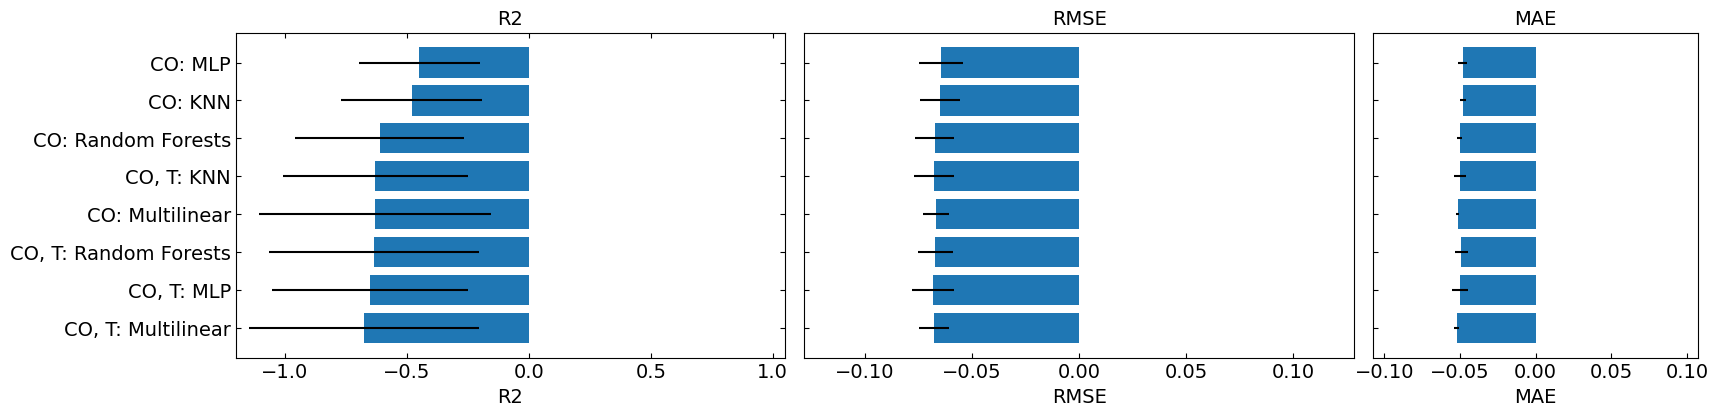
\includegraphics[width=\textwidth]{chapters/3-ANÁLISE DOS DADOS/Figuras/co-b4-models-performance.png}
    \label{fig:data-co-b4-models-performance}
\end{figure}

Como se observa todas as variantes de modelos e variáveis de entrada apresentaram valores de R2 negativos, indicando que nenhum dos modelos foi capaz de explicar a variância na variável dependente, i.e. a concentração real. Contudo, os modelos não lineares que incluíram a temperatura como variável de entrada, apresentaram melhorias na correlação entre a concentração real e a medida pelo sensor, com coeficientes de correlação de até 0.51. As Figuras \ref{fig:data-co-T-reference-corr-KNN} e \ref{fig:data-co-T-reference-corr-RF} apresentam os resultados ao aplicar os modelos de k Vizinhos mais Próximos e Florestas Aleatórias.

\begin{figure}[h]
    \centering
    \caption{Gráfico de dispersão das leituras do sensor CO-B4 e a estação de referência após aplicar modelos de regressão considerando a temperatura}
    \begin{subfigure}{0.49\textwidth}
        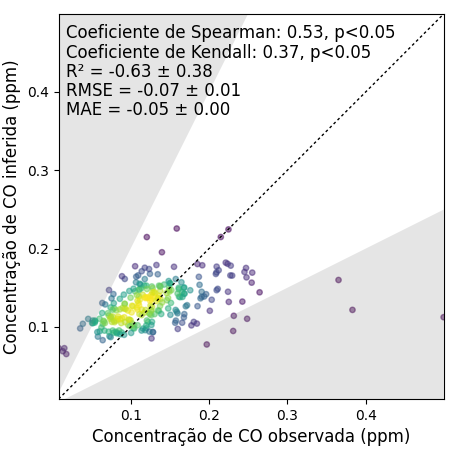
\includegraphics[width=\textwidth]{chapters/3-ANÁLISE DOS DADOS/Figuras/co-b4-T-KNN-Regression.png}
        \caption{Utilizando regressão pelos k Vizinhos mais Próximos}
        \label{fig:data-co-T-reference-corr-KNN}
    \end{subfigure}
    \hfill
    \begin{subfigure}{0.49\textwidth}
        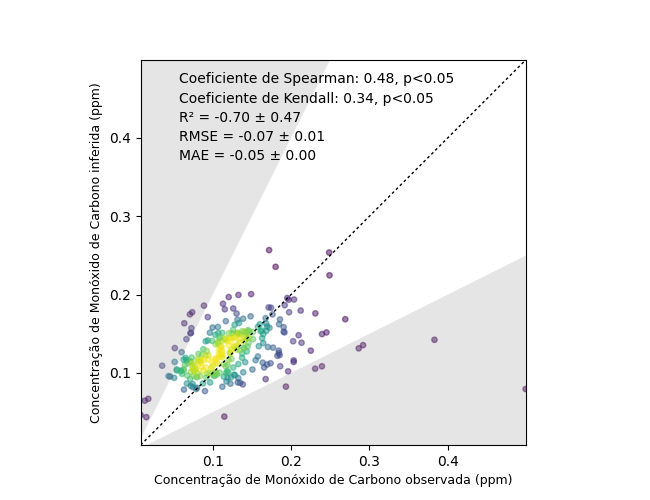
\includegraphics[width=\textwidth]{chapters/3-ANÁLISE DOS DADOS/Figuras/co-b4-T-RF-Regression.png}
        \caption{Utilizando regressão pelas Florestas Aleatórias}
        \label{fig:data-co-T-reference-corr-RF}
    \end{subfigure}
\end{figure}


% ----------------------------------------------------------
\section{Análise dos dados de Ozônio}
% ----------------------------------------------------------

Para a medição de \acrshort{o3} foram utilizados dois sensores do modelo OX-B431. As Figuras \ref{fig:data-o3-1-raw} e \ref{fig:data-o3-2-raw} mostram as séries temporais dos sensores depois de removidos os valores fora de intervalo. Observa-se que o sensor 1 sofreu alterações no valor de linha base nos meses de dezembro, fevereiro, março e abril, que foram detectadas pelo algoritmo \acrshort{pelt}, conforme ilustrado na Figura \ref{fig:data-rebase-o3-1}. As amostras dentro dos intervalos que apresentaram variações na linha base no sensor 1 foram etiquetados correspondentemente para sua remoção. As leituras do sensor 2 não apresentaram alterações na linha base.

\begin{figure}[h]
    \centering
    \caption{Série temporal dos sensores de \acrshort{o3} modelo OX-B431}
    \begin{subfigure}{0.495\textwidth}
        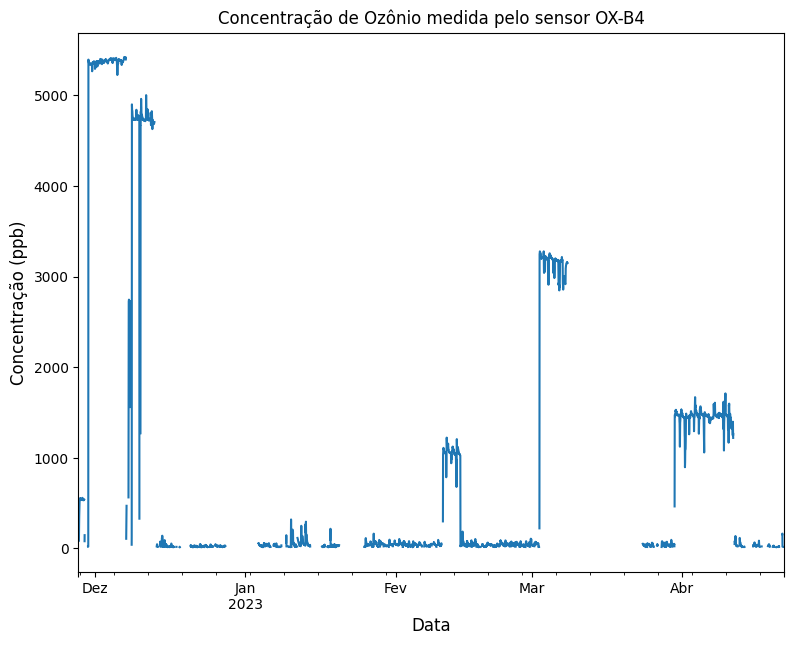
\includegraphics[width=\textwidth]{chapters/3-ANÁLISE DOS DADOS/Figuras/raw-o3-b4-1.png}
        \caption{Série temporal do sensor 1 depois de remover valores fora de intervalo}
        \label{fig:data-o3-1-raw}
    \end{subfigure}
    \hfill
    \begin{subfigure}{0.495\textwidth}
        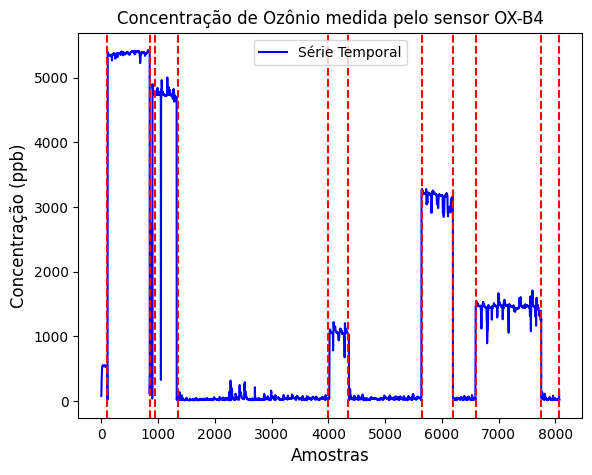
\includegraphics[width=\textwidth]{chapters/3-ANÁLISE DOS DADOS/Figuras/rebase-o3-b4-1.png}
        \caption{Pontos de alteração da linha base no sensor 1 detectados pelo algoritmo \acrshort{pelt}}
        \label{fig:data-rebase-o3-1}
    \end{subfigure}
    \hfill
    \begin{subfigure}{0.495\textwidth}
        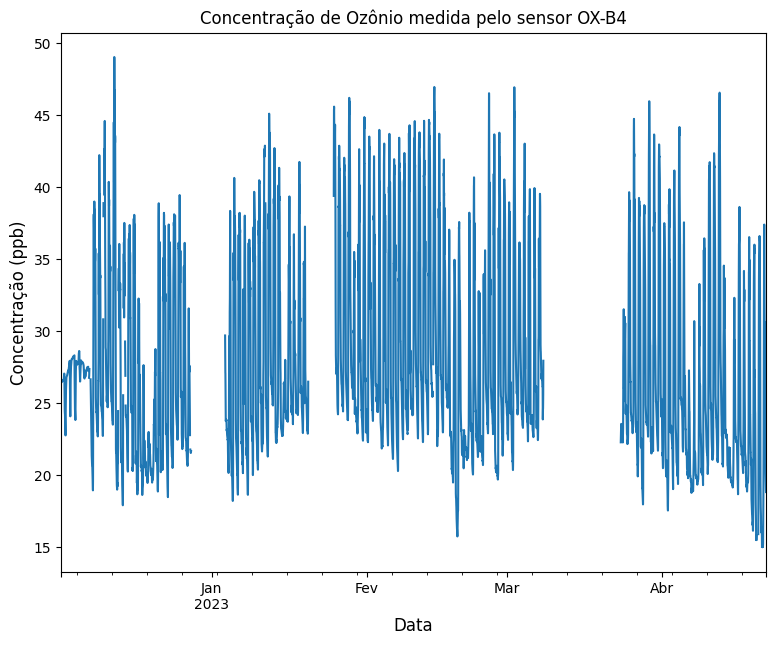
\includegraphics[width=\textwidth]{chapters/3-ANÁLISE DOS DADOS/Figuras/raw-o3-b4-2.png}
        \caption{Série temporal do sensor 2 depois de remover valores fora de intervalo}
        \label{fig:data-o3-2-raw}
    \end{subfigure}
    \label{fig:data-o3-raw-and-pelt}
    \fonte{Desenvolvido pelo autor (2023)}
\end{figure}

Depois de pré-processadas as leituras dos sensores de ozônio obtiveram-se os resultados ilustrados nas Figuras \ref{fig:data-o3-1-preproc-15} e \ref{fig:data-o3-2-preproc-15}. Os gráficos mostram as séries dos dados pré-processados dos dois sensores OX-B431 juntamente com o comportamento diário das medições ao longo do período, agrupados por hora do dia. Na Figura \ref{fig:data-o3-reference} observa-se uma clara componente diária nas leituras de concentração, que coincide com o comportamento apresentado pelas medições de referência (Figura \ref{fig:data-o3-reference}). Esse comportamento é esperado nas medições de \acrshort{o3} já que a variável é influenciada pela luz solar.

\begin{figure}[h]
    \centering
    \caption{Séries temporais dos sensores OX-B431 pré-processadas}
    \begin{subfigure}{0.95\textwidth}
        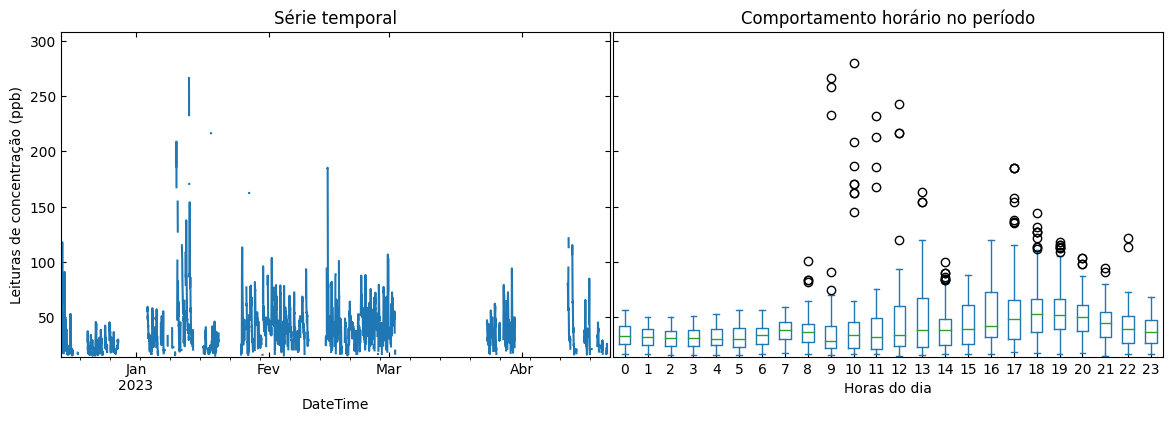
\includegraphics[width=\textwidth]{chapters/3-ANÁLISE DOS DADOS/Figuras/preproc-ox-b4-1.png}
        \caption{Série temporal do sensor 1 pré-processada (T = 15 mins) e seu comportamento diário}
        \label{fig:data-o3-1-preproc-15}
    \end{subfigure}
    \begin{subfigure}{0.95\textwidth}
        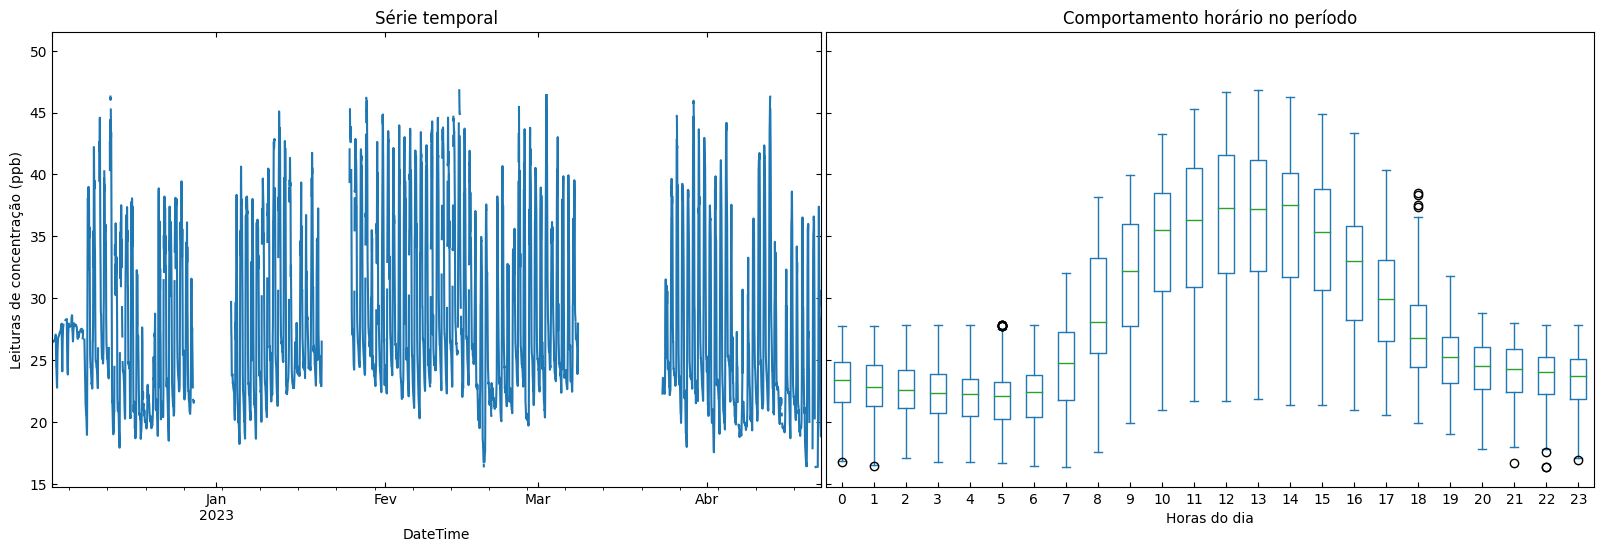
\includegraphics[width=\textwidth]{chapters/3-ANÁLISE DOS DADOS/Figuras/preproc-ox-b4-2.png}
        \caption{Série temporal do sensor 2 pré-processada (T = 15 mins) e seu comportamento diário}
        \label{fig:data-o3-2-preproc-15}
    \end{subfigure}
    \label{fig:data-o3-preproc-15}
    \begin{subfigure}{0.95\textwidth}
        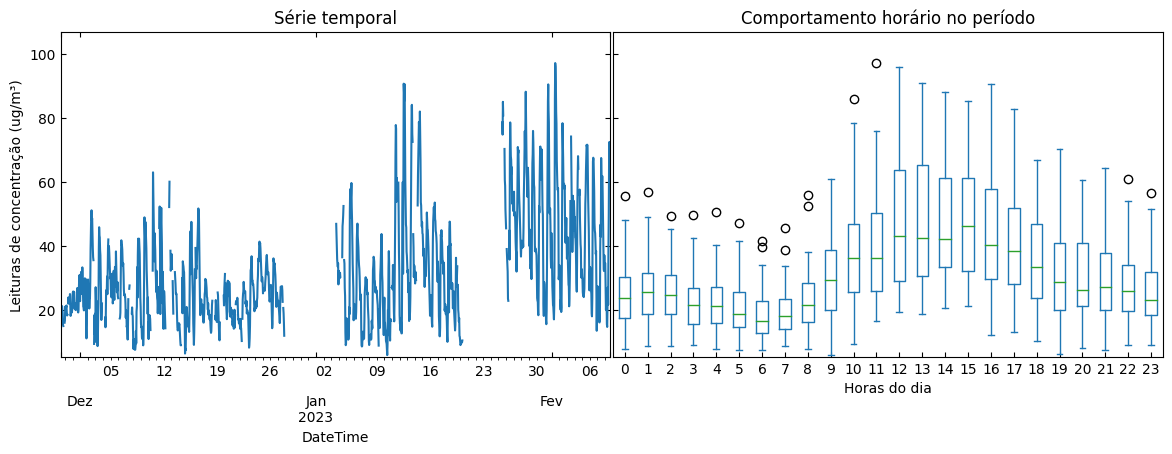
\includegraphics[width=\textwidth]{chapters/3-ANÁLISE DOS DADOS/Figuras/o3-reference-series-and-box.png}
        \caption{Série temporal das leituras de concentração de referência (T = 1 H) e seu comportamento diário}
        \label{fig:data-o3-reference}
    \end{subfigure}
    \label{fig:data-o3-preproc-15}
\end{figure}

Histogramas das leituras dos sensores OX-B431 são mostrados nas Figuras \ref{fig:data-o3-1-preproc-hist} e \ref{fig:data-o3-2-preproc-hist}. Os dados adquiridos pelo sensor 1 apresentaram um comportamento log-normal. Já o sensor 2 produziu leituras com uma componente log-normal e uma outra componente de menor frequência nos valores de concentração acima 30 ppb. Esta última representa a componente com sazonalidade diária mencionada acima. As séries re-amostradas em períodos de 1 hora são mostradas nas Figuras \ref{fig:data-o3-1-preproc-1HR} e \ref{fig:data-o3-2-preproc-1HR}.

\begin{figure}[h]
    \centering
    \caption{Histogramas e séries temporais horárias das leituras dos sensores OX-B431}
    \begin{subfigure}{0.495\textwidth}
        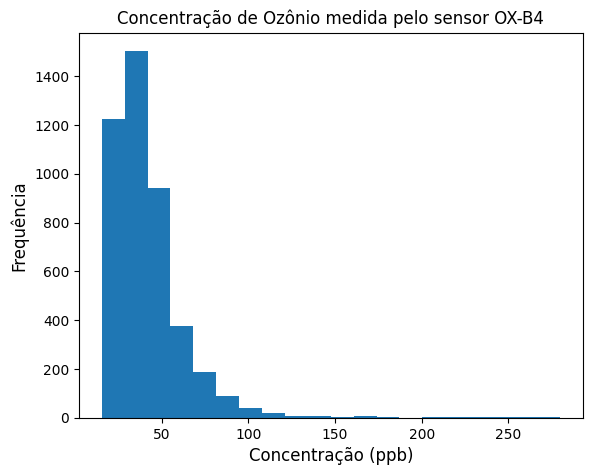
\includegraphics[width=\textwidth]{chapters/3-ANÁLISE DOS DADOS/Figuras/preproc-hist-ox-b4-1.png}
        \caption{Histograma das leituras do sensor 1 OX-B431}
        \label{fig:data-o3-1-preproc-hist}
    \end{subfigure}
    \hfill
    \begin{subfigure}{0.495\textwidth}
        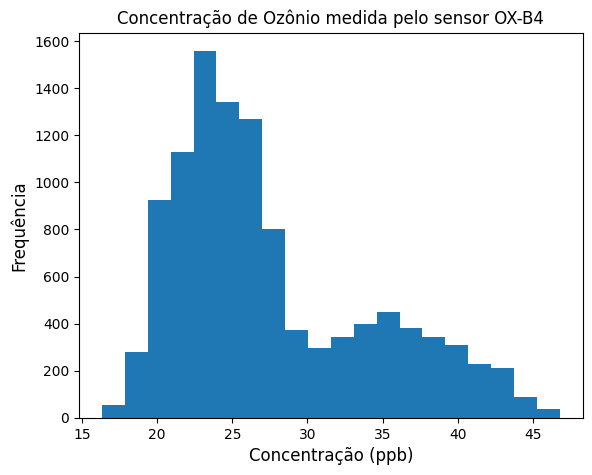
\includegraphics[width=\textwidth]{chapters/3-ANÁLISE DOS DADOS/Figuras/preproc-hist-ox-b4-2.png}
        \caption{Histograma das leituras do sensor 2 OX-B431}
        \label{fig:data-o3-2-preproc-hist}
    \end{subfigure}
    \hfill
    \begin{subfigure}{0.495\textwidth}
        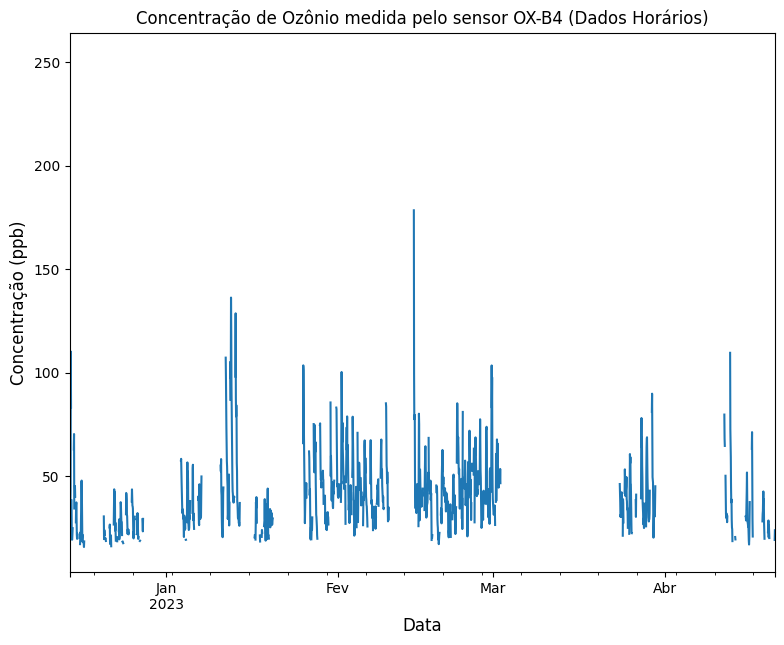
\includegraphics[width=\textwidth]{chapters/3-ANÁLISE DOS DADOS/Figuras/preproc-1HR-ox-b4-1.png}
        \caption{Série temporal do sensor 2 com T = 1 hr}
        \label{fig:data-o3-1-preproc-1HR}
    \end{subfigure}
    \hfill
    \begin{subfigure}{0.495\textwidth}
        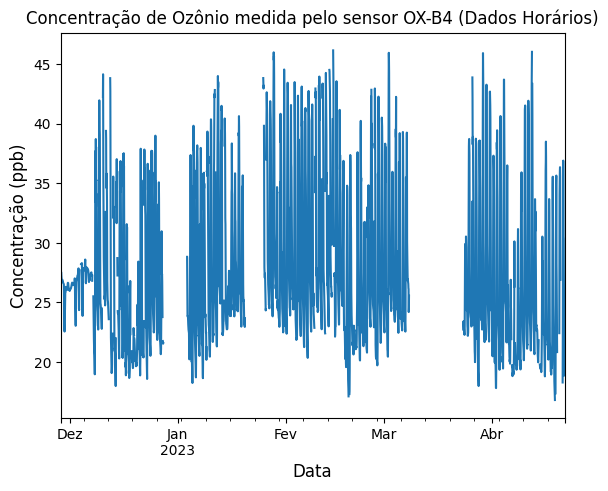
\includegraphics[width=\textwidth]{chapters/3-ANÁLISE DOS DADOS/Figuras/preproc-1HR-ox-b4-2.png}
        \caption{Série temporal do sensor 2 com T = 1 hr}
        \label{fig:data-o3-2-preproc-1HR}
    \end{subfigure}
    \fonte{Desenvolvido pelo autor (2023)}
\end{figure}

Nas Tabelas \ref{tab:data-contab-o3-1} e \ref{tab:data-contab-o3-2} contabilizam-se os dados dos sensores de \acrshort{o3} para períodos de 15 minutos e de 1 hora. Observa-se que no sensor 1, dos 14625 pontos de dados, que representavam as amostras adquiridas com um período de 15 minutos no intervalo de 20/11/2022 até 21/04/2023, 4413 foram aproveitados como dados válidos, o que representa um 30 \% aproximadamente dos dados originais. Ao re-amostrar esses 4413 pontos em dados horários obtiveram-se 1056 amostras horárias de concentração válidas (aproximadamente 34 \% dos dados) para realizar a calibração. Já no sensor 2, dos 14542 pontos de dados, que representavam as amostras adquiridas no intervalo de 21/11/2022 até 21/04/2023, 10814 foram aproveitados como dados válidos, o que representa um 74 \% aproximadamente dos dados originais. Ao re-amostrar esses 10814 pontos válidos em dados horários obtiveram-se 2685 amostras horárias de concentração válidas (aproximadamente 77 \% dos dados) para realizar a calibração.

\begin{table}[h]
    \caption{Contabilização dos dados por etiquetas das leituras do sensor 1 OX-B431}
    \centering
    \begin{tabularx}{0.95\textwidth}[h]{
         >{\raggedright\hsize=.475\hsize\arraybackslash}X
         >{\raggedright\hsize=.20\hsize\arraybackslash}X 
         >{\raggedright\hsize=.5\hsize\arraybackslash}X
        | >{\raggedright\hsize=.50\hsize\arraybackslash}X 
         >{\raggedright\hsize=.20\hsize\arraybackslash}X 
         >{\raggedright\hsize=.5\hsize\arraybackslash}X }
        \multicolumn{3}{c|}{Série temporal T = 15 mins} & \multicolumn{3}{c}{Série temporal T = 1 hr} \\
        \hline
        Etiquetas & No. amostras & \% amostras & Etiquetas & No. amostras & \% amostras \\ [0.5ex]
        \hline
        \textit{MISSING} & 2750 & 18.80 \% & \textit{LOWSAMPLES} & 2020 & 65.67 \% \\ [0.5ex]
        
        \textit{LTLL} & 3134 & 21.43 \% & \textit{VALID} & 1056 & 34.33 \% \\ [0.5ex]
        
        \textit{GTUL} & 0 & 0.0 \% & & & \\ [0.5ex]
        
        \textit{STABILIZING} & 514 & 3.51 \% & & & \\ [0.5ex]
        
        \textit{BADSPIKE} & 56 & 0.38 \% & & & \\ [0.5ex]
        
        \textit{LTQTLE01} & 102 & 0.70 \% & & & \\ [0.5ex]
        
        \textit{GTQTLE99} & 64 & 0.44 \% & & & \\ [0.5ex]
        
        \textit{REBASE} & 3592 & 24.56 \% & & & \\ [0.5ex]

        \textit{VALID} & 4413 & 30.17 \% & & & \\ [0.5ex]
        \hline
        TOTAL & 14625 & & TOTAL & 3076 & \\
    \end{tabularx}
    \label{tab:data-contab-o3-1}
    \fonte{Desenvolvido pelo autor}
\end{table}

\begin{table}[h]
    \caption{Contabilização dos dados por etiquetas das leituras do sensor 2 OX-B431}
    \centering
    \begin{tabularx}{0.95\textwidth}[h]{
         >{\raggedright\hsize=.475\hsize\arraybackslash}X
         >{\raggedright\hsize=.20\hsize\arraybackslash}X 
         >{\raggedright\hsize=.5\hsize\arraybackslash}X
        | >{\raggedright\hsize=.50\hsize\arraybackslash}X 
         >{\raggedright\hsize=.20\hsize\arraybackslash}X 
         >{\raggedright\hsize=.5\hsize\arraybackslash}X }
        \multicolumn{3}{c|}{Série temporal T = 15 mins} & \multicolumn{3}{c}{Série temporal T = 1 hr} \\
        \hline
        Etiquetas & No. amostras & \% amostras & Etiquetas & No. amostras & \% amostras \\ [0.5ex]
        \hline
        \textit{MISSING} & 2734 & 18.80 \% & \textit{LOWSAMPLES} & 783 & 22.58 \% \\ [0.5ex]
        
        \textit{LTLL} & 49 & 0.34 \% & \textit{VALID} & 2685 & 77.42 \% \\ [0.5ex]
        
        \textit{GTUL} & 0 & 0.0 \% & & & \\ [0.5ex]
        
        \textit{STABILIZING} & 673 & 4.63 \% & & & \\ [0.5ex]
        
        \textit{BADSPIKE} & 0 & 0.0 \% & & & \\ [0.5ex]
        
        \textit{LTQTLE01} & 125 & 0.86 \% & & & \\ [0.5ex]
        
        \textit{GTQTLE99} & 147 & 1.01 \% & & & \\ [0.5ex]
        
        \textit{REBASE} & 0 & 0.0 \% & & & \\ [0.5ex]
        
        \textit{VALID} & 10814 & 74.36 \% & & & \\ [0.5ex]
        \hline
        TOTAL & 14542 & & TOTAL & 3468 & \\
    \end{tabularx}
    \label{tab:data-contab-o3-2}
    \fonte{Desenvolvido pelo autor}
\end{table}

\subsection{Dependência com a temperatura}

Investigou-se a existência de correlação entre as leituras dos sensores de \acrshort{o3} e as variações de temperatura medida no interior da câmara de medição. Os resultados dos testes estatísticos de Spearman e Kendall revelaram coeficientes de correlação significativos, conforme se ilustra nas Figuras \ref{fig:data-temp-o3-1-corr} e \ref{fig:data-temp-o3-2-corr}. Os coeficientes de Spearman calculados foram de 0.37 e 0.85 para os sensores 1 e 2 respectivamente, com valores de p inferiores a 0.05, indicando uma correlação estatisticamente significativa entre as leituras dos sensores e a temperatura. De maneira semelhante, os coeficientes de Kendall foram de 0.27 e 0.70 respectivamente, também com p < 0.05, reforçando a presença de uma associação significativa. Ao avaliar a hipótese nula de ausência de correlação, os resultados forneceram evidências para sua rejeição, sugerindo a existência de uma correlação entre as leituras dos sensores de \acrshort{o3} e as variações de temperatura.

\begin{figure}[h]
    \centering
    \caption{Relação entre as leituras dos sensores de \acrshort{o3} e a temperatura}
    \begin{subfigure}{0.495\textwidth}
        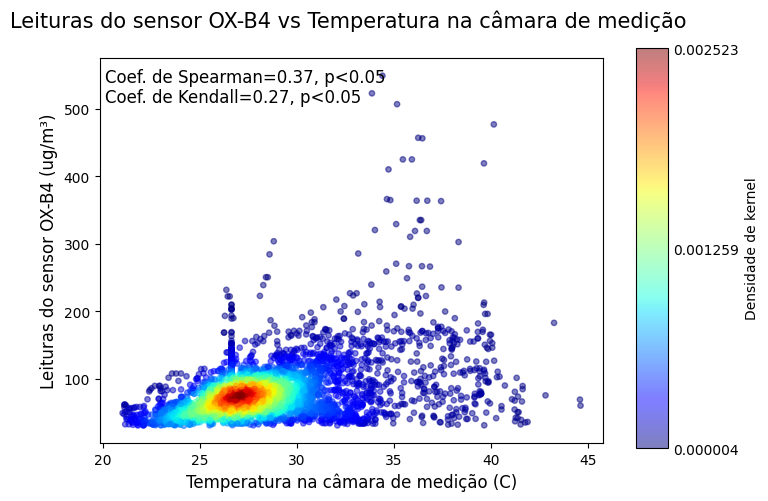
\includegraphics[width=\textwidth]{chapters/3-ANÁLISE DOS DADOS/Figuras/temperature-o3-b4-1.png}
        \caption{Relação entre as leituras do sensor 1 de \acrshort{o3} e a temperatura}
        \label{fig:data-temp-o3-1-corr}    
    \end{subfigure}
    \hfill
    \begin{subfigure}{0.495\textwidth}
        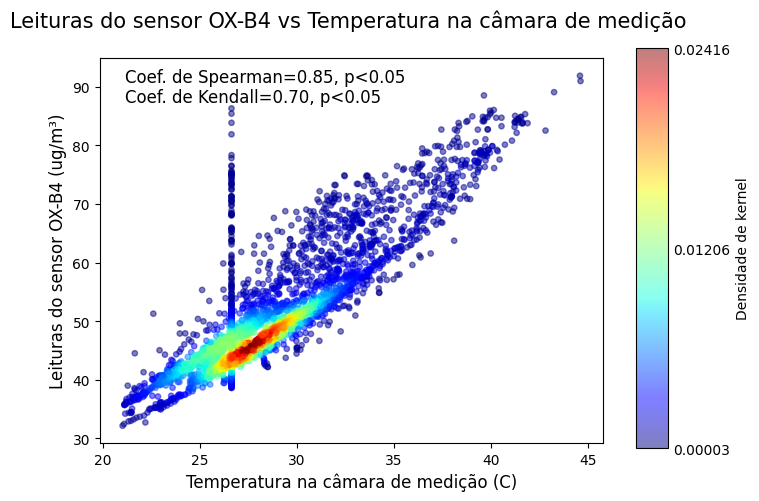
\includegraphics[width=\textwidth]{chapters/3-ANÁLISE DOS DADOS/Figuras/temperature-o3-b4-2.png}
        \caption{Relação entre as leituras do sensor 2 de \acrshort{o3} e a temperatura}
        \label{fig:data-temp-o3-2-corr}    
    \end{subfigure}
    \hfill
    \begin{subfigure}{0.495\textwidth}
        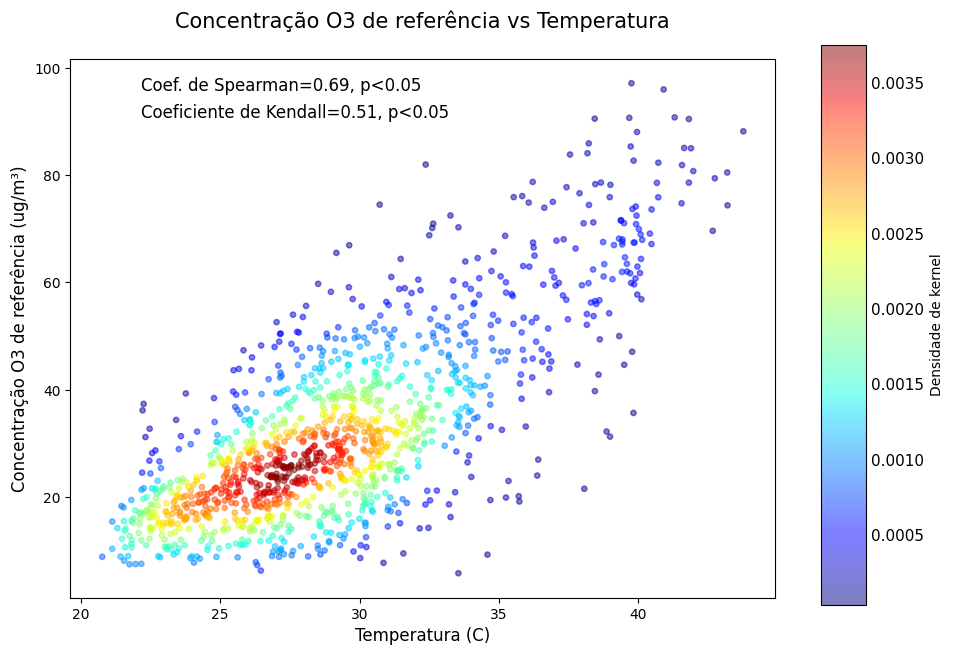
\includegraphics[width=\textwidth]{chapters/3-ANÁLISE DOS DADOS/Figuras/temperature-o3-reference.png}
        \caption{Relação entre os valores de concentração de referência e a temperatura}
        \label{fig:data-temp-o3-ref-corr}    
    \end{subfigure}
    \label{fig:data-temp-o3-corr}
\end{figure}

Os resultados obtidos nos testes estatísticos podem ser corroborados nos gráficos de dispersão entre as variáveis nas Figuras \ref{fig:data-temp-o3-1-corr} e \ref{fig:data-temp-o3-2-corr}. Delas comprova-se uma maior correlação com a temperatura no sensor 2, que coincide com o comportamento sazonal diário observado anteriormente. As leituras de referência também apresentaram uma relação linear com a temperatura, com coeficientes de Spearman e Kendall de 0.69 e 0.51 respectivamente, conforme se ilustra na Figura \ref{fig:data-temp-o3-ref-corr}.

\subsection{Calibração das leituras dos sensores OX-B431 com as medições de referência}

Nas Figuras \ref{fig:data-o3-reference-time-series}, \ref{fig:data-o3-1-reference-corr} e \ref{fig:data-o3-2-reference-corr} apresentam-se as leituras de \acrshort{o3} obtidas pelos sensores OX-B431 de Alphasense e a estação de referência. Observa-se que as leituras do sensor 1 superestimaram os valores de concentração de referência. Os testes de Spearman e Kendall revelaram a existência de correlação entre as medições com o sensor 1 e a referência com coeficientes de 0.38 e 0.27 respectivamente, e de 0.59 e 0.42 respectivamente para o sensor 2.

\begin{figure}[h]
    \centering
    \caption{Séries temporais e gráficos de dispersão das medições de \acrshort{o3}}
    \begin{subfigure}{0.4\textwidth}
        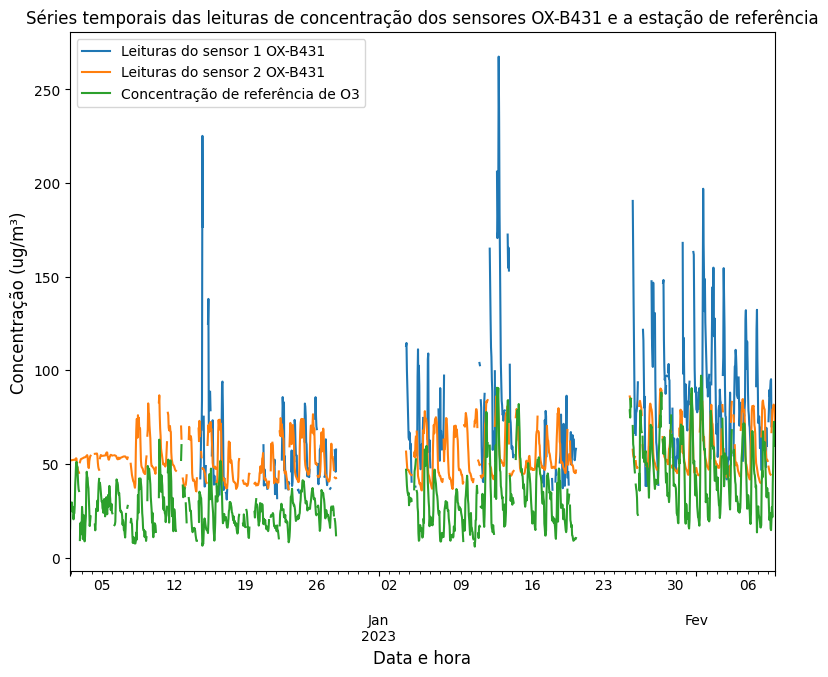
\includegraphics[width=\textwidth]{chapters/3-ANÁLISE DOS DADOS/Figuras/o3-b4-reference-time-series.png}
        \caption{Séries temporais das leituras dos sensores OX-B431 e a estação de referência}
        \label{fig:data-o3-reference-time-series}
    \end{subfigure}
    \hfill
    \begin{subfigure}{0.5\textwidth}
        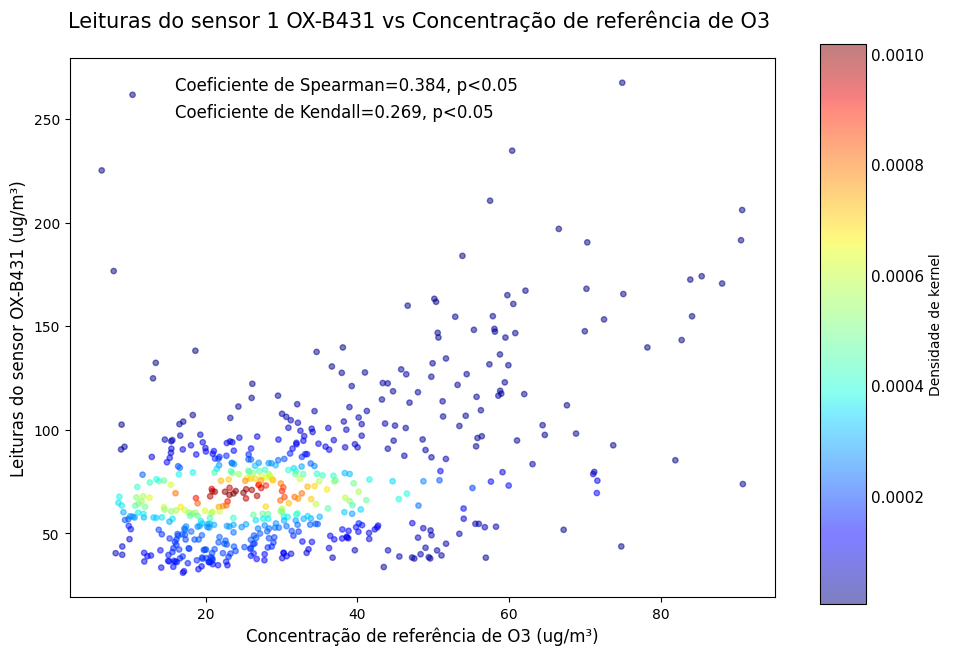
\includegraphics[width=\textwidth]{chapters/3-ANÁLISE DOS DADOS/Figuras/o3-b4-1-reference-correlation.png}
        \caption{Gráfico de dispersão das leituras do sensor 1 OX-B431 e a estação de referência}
        \label{fig:data-o3-1-reference-corr}
    \end{subfigure}
    \hfill
    \begin{subfigure}{0.5\textwidth}
        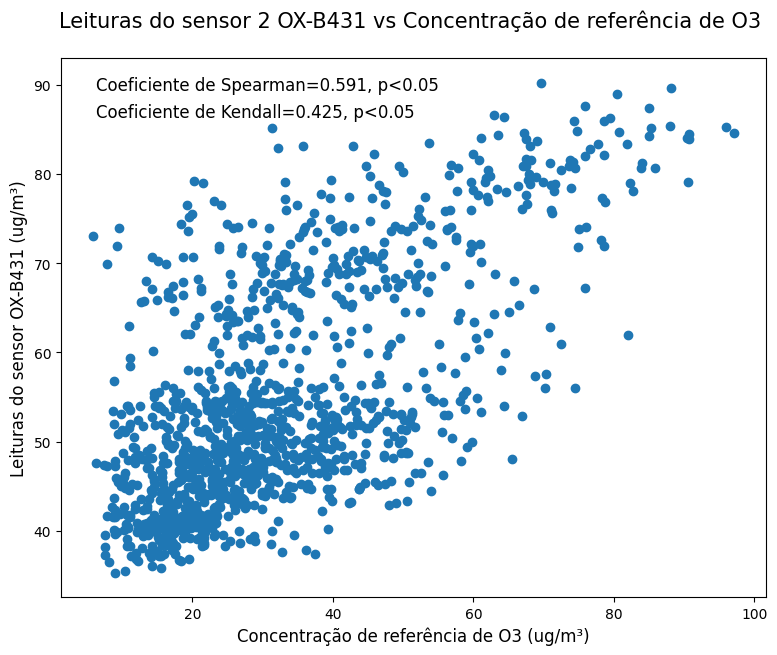
\includegraphics[width=\textwidth]{chapters/3-ANÁLISE DOS DADOS/Figuras/o3-b4-2-reference-correlation.png}
        \caption{Gráfico de dispersão das leituras do sensor 2 OX-B431 e a estação de referência}
        \label{fig:data-o3-2-reference-corr}
    \end{subfigure}
\end{figure}

\begin{figure}[h!]
    \centering
    \caption{Resultados dos modelos de calibração aplicados às leituras dos sensores OX-B431}
    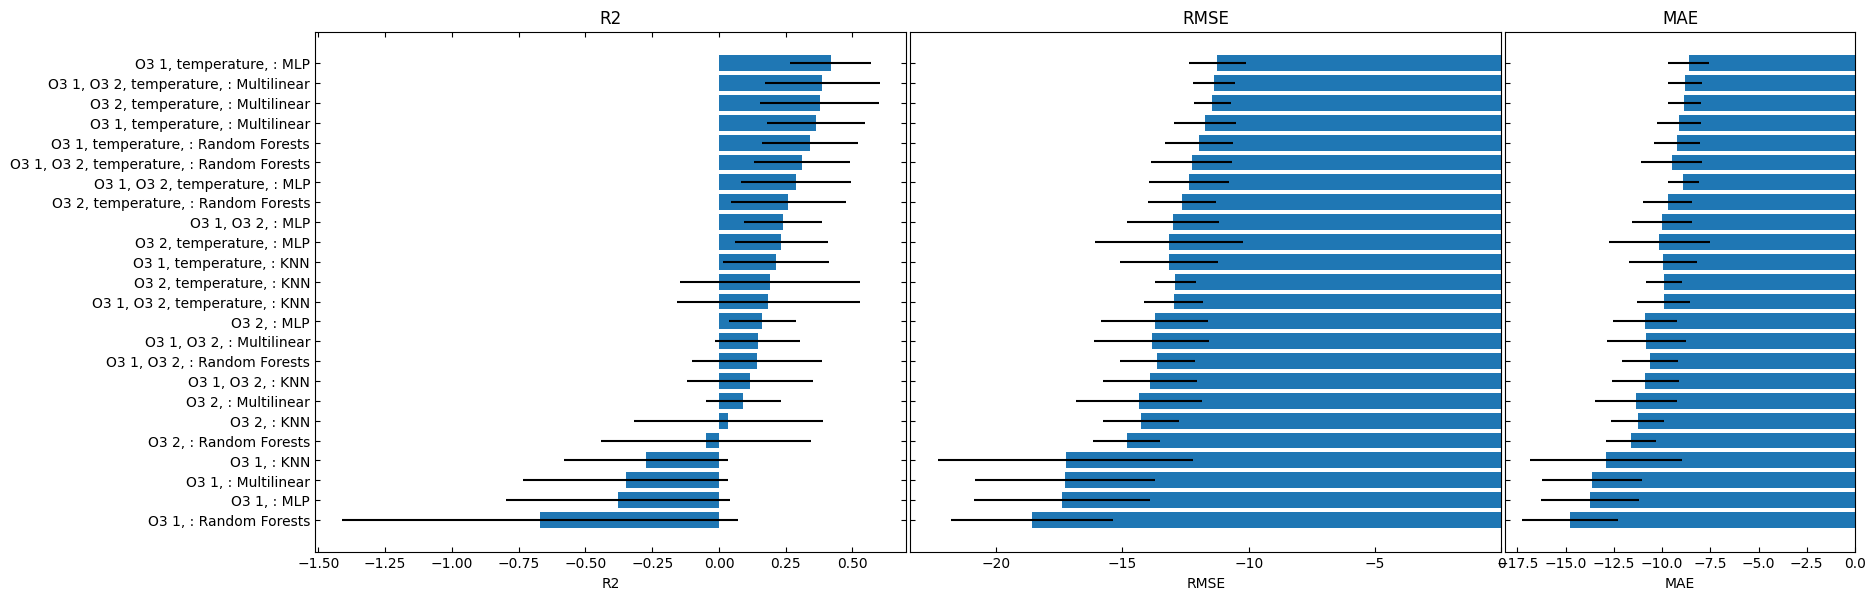
\includegraphics[width=\textwidth]{chapters/3-ANÁLISE DOS DADOS/Figuras/o3-b4-models-performance.png}
    \label{fig:data-o3-b4-models-performance}
\end{figure}

A partir dos dados de referência e das leituras de concentração e temperatura adquiridas pelo monitor em questão, foi realizada uma busca em grid para encontrar as melhores combinações de parâmetros e variáveis de entrada a modelos de regressão. As variáveis que foram testadas como entrada foram as leituras de concentração de \acrshort{o3} dos dois sensores OX-B431 e a temperatura no interior da câmara de medição. Como modelos de regressão foram testados: o Perceptron Multicamadas (MLP), a Regressão Linear Multivariada (MLR), os K Vizinhos mais Próximos (KNN) e as Florestas Aleatórias (RF). Nas Tabelas \ref{tab:data-o3-1-b4-calib-results} - \ref{tab:data-o3-1-2-b4-calib-results} resumem-se os melhores modelos encontrados pela busca em \textit{grid} para calibrar as leituras dos sensores OX-B431. A Tabela \ref{tab:data-o3-1-b4-calib-results} apresenta os modelos obtidos considerando o sensor 1 e a temperatura. A Tabela \ref{tab:data-o3-2-b4-calib-results} compila os mesmos parâmetros para o sensor 2 e a temperatura. Já a Tabela \ref{tab:data-o3-1-2-b4-calib-results} resume os modelos obtidos ao considerar como variáveis independentes ambos sensores e a temperatura. Os mesmos resultados são ilustrados graficamente na Figura \ref{fig:data-o3-b4-models-performance} que apresenta o desempenho dos modelos e as variáveis de entrada considerando os valores de r2, RMSE e MAE.

\begin{figure}[h!]
    \centering
    \caption{Gráfico de dispersão das leituras dos sensores de \acrshort{o3} OX-B431 e a estação de referência após aplicar modelos de regressão considerando a temperatura}
    \begin{subfigure}{0.49\textwidth}
        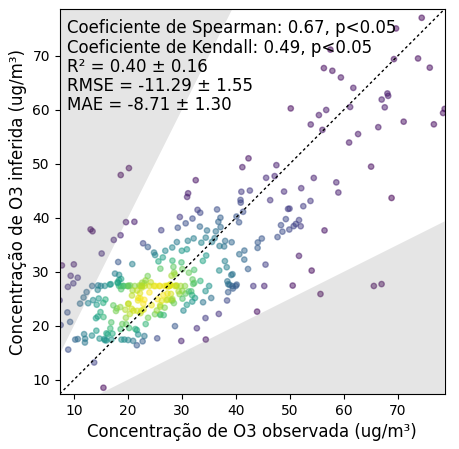
\includegraphics[width=\textwidth]{chapters/3-ANÁLISE DOS DADOS/Figuras/o3-b4-1-T-MLP-Regression.png}
        \caption{Utilizando uma rede neural Perceptron Multicamadas obtiverem-se os melhores resultados de R2, RMSE e MAE considerando as leituras do sensor 1 e a temperatura}
        \label{fig:data-o3-1-T-reference-corr-MLP}
    \end{subfigure}
    \hfill
    \begin{subfigure}{0.49\textwidth}
        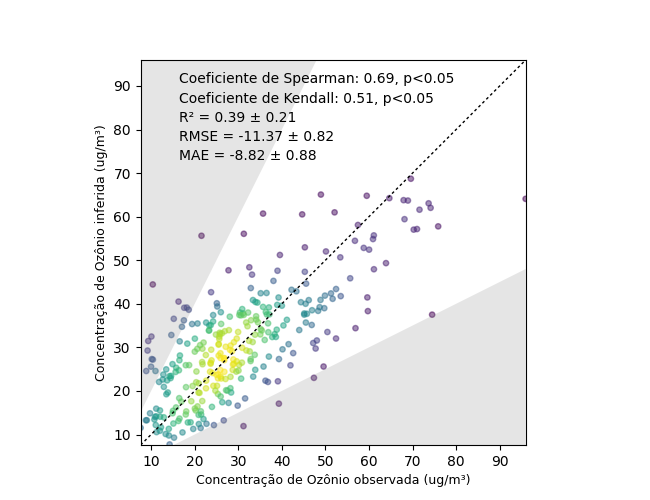
\includegraphics[width=\textwidth]{chapters/3-ANÁLISE DOS DADOS/Figuras/o3-b4-1-2-T-Multilinear-Regression.png}
        \caption{Utilizando uma regressão linear considerando as leituras dos sensores e a temperatura obtiveram-se resultados semelhantes}
        \label{fig:data-o3-1-2-T-reference-corr-MLR}
    \end{subfigure}
\end{figure}

De modo geral observa-se que os modelos que consideraram a temperatura como variável de entrada produziram os melhores resultados de r2, erro e correlação. Ao considerar os sensores de ozônio de forma independente, os resultados dos modelos não foram bons, com o sensor 2 gerando melhores resultados do que o sensor 1 (correlação e r2 maiores). Quando consideradas as leituras de ambos sensores, os modelos geraram melhores resultados, embora inferiores a quando considerada a temperatura. As Figuras \ref{fig:data-o3-1-T-reference-corr-MLP} e \ref{fig:data-o3-1-2-T-reference-corr-MLR} apresentam gráficos de dispersão com as leituras de referência e as inferidas pelos dois melhores modelos em termos de R2, RMSE e MAE.

\begin{table}[h]
    \caption{Resultados da calibração do sensor 1 OX-B431}
    \centering
    \begin{tabularx}{0.95\textwidth}[h!]{
        >{\raggedright\hsize=.2\hsize\arraybackslash}X
        >{\raggedright\hsize=.7\hsize\arraybackslash}X 
        >{\raggedright\hsize=.4\hsize\arraybackslash}X
        >{\raggedright\hsize=.4\hsize\arraybackslash}X 
        >{\raggedright\hsize=.3\hsize\arraybackslash}X 
        >{\raggedright\hsize=.3\hsize\arraybackslash}X }
       \hline
       Var. & Modelo & R2 & RMSE & MAE & $\rho$\\ [0.5ex]
        \hline
        \acrshort{o3} (1) & \textbf{MLP}: & -0.38 ± 0.42 & -17.38 ± 3.49 & -13.72 ± 2.55 & 0.21 \\ [0.5ex]
           & alpha = 0.0001 &  & & & \\ [0.5ex]
           & hidden layers = (100,) & & & & \\ [0.5ex]
           & & & & & \\ [0.5ex]
           & \textbf{MLR} & -0.35 ± 0.38 & -17.26 ± 3.57 & -13.63 ± 2.58 & 0.22 \\ [0.5ex]
           & & & & & \\ [0.5ex]
           & \textbf{KNN:} & -0.27 ± 0.31 & -17.24 ± 5.05 & -12.91 ± 3.92 & 0.21 \\ [0.5ex]
           & n\_neighbors = 13 & & & & \\ [0.5ex]
           & weights = uniform & & & & \\ [0.5ex]
           & & & & & \\ [0.5ex]
           & \textbf{RF:} & -0.68 ± 0.73 & -18.65 ± 3.27 & -14.87 ± 2.54 & 0.17 \\ [0.5ex]
           & max\_depth = 20 & & & & \\ [0.5ex]
           & min\_samples\_leaf = 4 & & & & \\ [0.5ex]
           & min\_samples\_split = 10 & & & & \\ [0.5ex]
           & n\_estimators = 50 & & & & \\ [0.5ex]
        \hline
        \acrshort{o3} (1), T & \textbf{MLP:} & 0.42 ± 0.15 & -11.24 ± 1.13 & -8.62 ± 1.07 & 0.69 \\ [0.5ex]
            & alpha = 0.0001 & & & & \\ [0.5ex]
            & hidden layer = (200, 10) & & & & \\ [0.5ex]
            & & & & & \\ [0.5ex]
            & \textbf{MLR:} & 0.36 ± 0.18 & -11.73 ± 1.23 & -9.12 ± 1.12 & 0.67 \\ [0.5ex]
            & & & & & \\ [0.5ex]
            & \textbf{KNN:} & 0.21 ± 0.20 & -13.16 ± 1.93 & -9.96 ± 1.76 & 0.66 \\ [0.5ex]
            & n\_neighbors = 7 & & & & \\ [0.5ex]
            & weights = uniform & & & & \\ [0.5ex]
            & & & & & \\ [0.5ex]
            & \textbf{RF:} & 0.33 ± 0.19 & -11.99 ± 1.23 & -9.24 ± 1.12 & 0.62 \\ [0.5ex]
            & max\_depth = 10 & & & & \\ [0.5ex]
            & min\_samples\_leaf = 4 & & & & \\ [0.5ex]
            & min\_samples\_split = 10 & & & & \\ [0.5ex]
            & n\_estimators = 100 & & & & \\ [0.5ex]
        \hline
    \end{tabularx}
    \label{tab:data-o3-1-b4-calib-results}
\end{table}

\begin{table}[h]
    \caption{Resultados da calibração do sensor 2 OX-B431}
    \centering
    \begin{tabularx}{0.95\textwidth}[h!]{
        >{\raggedright\hsize=.2\hsize\arraybackslash}X
        >{\raggedright\hsize=.7\hsize\arraybackslash}X 
        >{\raggedright\hsize=.4\hsize\arraybackslash}X
        >{\raggedright\hsize=.4\hsize\arraybackslash}X 
        >{\raggedright\hsize=.3\hsize\arraybackslash}X 
        >{\raggedright\hsize=.3\hsize\arraybackslash}X }
       \hline
       Var. & Modelo & R2 & RMSE & MAE & $\rho$\\ [0.5ex]
        \hline
        \acrshort{o3} (2) & \textbf{MLP}: & 0.16 ± 0.13 & -13.72 ± 2.11 & -10.87 ± 1.66 & 0.54 \\ [0.5ex]
           & alpha = 1 &  & & & \\ [0.5ex]
           & hidden layers = (50, 50) & & & & \\ [0.5ex]
           & & & & & \\ [0.5ex]
           & \textbf{MLR} & 0.09 ± 0.14 & -14.34 ± 2.50 & -11.35 ± 2.13 & 0.56 \\ [0.5ex]
           & & & & & \\ [0.5ex]
           & \textbf{KNN:} & 0.03 ± 0.35 & -14.27 +/- 1.49 & -11.27 ± 1.39 & 0.54 \\ [0.5ex]
           & n\_neighbors = 20 & & & & \\ [0.5ex]
           & weights = uniform & & & & \\ [0.5ex]
           & & & & & \\ [0.5ex]
           & \textbf{RF:} & -0.03 ± 0.37 & -14.76 ± 1.47 & -11.55 ± 1.34 & 0.52 \\ [0.5ex]
           & max\_depth = 10 & & & & \\ [0.5ex]
           & min\_samples\_leaf = 4 & & & & \\ [0.5ex]
           & min\_samples\_split = 10 & & & & \\ [0.5ex]
           & n\_estimators = 50 & & & & \\ [0.5ex]
        \hline
        \acrshort{o3} (2), T & \textbf{MLP:} & 0.23 ± 0.17 & -13.16 ± 2.94 & -10.14 ± 2.62 & 0.67 \\ [0.5ex]
            & alpha = 10 & & & & \\ [0.5ex]
            & hidden layer = (10, 10) & & & & \\ [0.5ex]
            & & & & & \\ [0.5ex]
            & \textbf{MLR:} & 0.38 ± 0.22 & -11.44 ± 0.72 & -8.86 ± 0.86 & 0.69 \\ [0.5ex]
            & & & & & \\ [0.5ex]
            & \textbf{KNN:} & 0.19 ± 0.34 & -12.91 ± 0.81 & -9.89 ± 0.92 & 0.70 \\ [0.5ex]
            & n\_neighbors = 2 & & & & \\ [0.5ex]
            & weights = uniform & & & & \\ [0.5ex]
            & & & & \\ [0.5ex]
            & \textbf{RF:} & 0.28 ± 0.22 & -12.44 ± 1.11 & -9.54 ± 1.08 & 0.67 \\ [0.5ex]
            & max\_depth = 10 & & & & \\ [0.5ex]
            & min\_samples\_leaf = 4 & & & & \\ [0.5ex]
            & min\_samples\_split = 10 & & & & \\ [0.5ex]
            & n\_estimators = 150 & & & & \\ [0.5ex]
        \hline
    \end{tabularx}
    \label{tab:data-o3-2-b4-calib-results}
\end{table}

\begin{table}[h]
    \caption{Resultados da calibração das leituras de \acrshort{o3} utilizando os sensores 1 e 2 OX-B431}
    \centering
    \begin{tabularx}{0.95\textwidth}[h!]{
        >{\raggedright\hsize=.2\hsize\arraybackslash}X
        >{\raggedright\hsize=.7\hsize\arraybackslash}X 
        >{\raggedright\hsize=.4\hsize\arraybackslash}X
        >{\raggedright\hsize=.4\hsize\arraybackslash}X 
        >{\raggedright\hsize=.3\hsize\arraybackslash}X 
        >{\raggedright\hsize=.3\hsize\arraybackslash}X }
       \hline
       Var. & Modelo & R2 & RMSE & MAE & $\rho$\\ [0.5ex]
        \hline
        \acrshort{o3} (1), \acrshort{o3} (2) & \textbf{MLP}: & 0.24 ± 0.15 & -13.01 ± 1.82 & -10.02 ± 1.55 & 0.60 \\ [0.5ex]
           & alpha = 1 &  & & & \\ [0.5ex]
           & hidden layers = (200, 4) & & & & \\ [0.5ex]
           & & & & & \\ [0.5ex]
           & \textbf{MLR} & 0.14 ± 0.16 & -13.85 ± 2.26 & -10.81 ± 2.02 & 0.58 \\ [0.5ex]
           & & & & & \\ [0.5ex]
           & \textbf{KNN:} & 0.12 ± 0.24 & -13.90 ± 1.86 & -10.86 ± 1.72 & 0.58 \\ [0.5ex]
           & n\_neighbors = 20 & & & & \\ [0.5ex]
           & weights = uniform & & & & \\ [0.5ex]
           & & & & & \\ [0.5ex]
           & \textbf{RF:} & 0.13 ± 0.24 & -13.70 ± 1.54 & -10.64 ± 1.43 & 0.57 \\ [0.5ex]
           & max\_depth = 10 & & & & \\ [0.5ex]
           & min\_samples\_leaf = 2 & & & & \\ [0.5ex]
           & min\_samples\_split = 10 & & & & \\ [0.5ex]
           & n\_estimators = 100 & & & & \\ [0.5ex]
        \hline
        \acrshort{o3} (1), \acrshort{o3} (2), T & \textbf{MLP:} & 0.29 ± 0.21 & -12.37 ± 1.59 & -8.89 ± 0.82 & 0.71 \\ [0.5ex]
            & alpha = 0.001 & & & & \\ [0.5ex]
            & hidden layer = (200,) & & & & \\ [0.5ex]
            & & & & & \\ [0.5ex]
            & \textbf{MLR:} & 0.39 ± 0.21 & -11.37 ± 0.82 & -8.82 ± 0.88 & 0.69 \\ [0.5ex]
            & & & & & \\ [0.5ex]
            & \textbf{KNN:} & 0.19 ± 0.34 & -12.97 ± 1.18 & -9.92 ± 1.37 & 0.72 \\ [0.5ex]
            & n\_neighbors = 13 & & & & \\ [0.5ex]
            & weights = distance & & & & \\ [0.5ex]
            & & & & & \\ [0.5ex]
            & \textbf{RF:} & 0.30 ± 0.19 & -12.34 ± 1.61 & -9.57 ± 1.58 & 0.68 \\ [0.5ex]
            & max\_depth = 10 & & & & \\ [0.5ex]
            & min\_samples\_leaf = 1 & & & & \\ [0.5ex]
            & min\_samples\_split = 10 & & & & \\ [0.5ex]
            & n\_estimators = 150 & & & & \\ [0.5ex]
        \hline
    \end{tabularx}
    \label{tab:data-o3-1-2-b4-calib-results}
\end{table}

% ----------------------------------------------------------
\section{Análise dos dados de Dióxido de Nitrogênio}
% ----------------------------------------------------------

\begin{figure}[h]
    \centering
    \caption{Série temporal do sensor NO2-B43F}
    \begin{subfigure}{0.495\textwidth}
        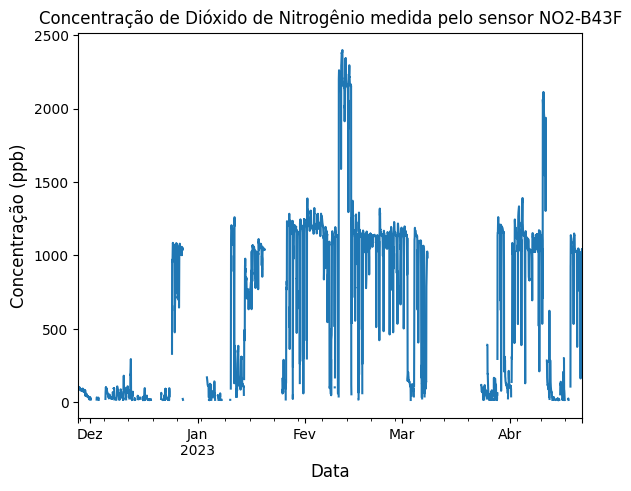
\includegraphics[width=\textwidth]{chapters/3-ANÁLISE DOS DADOS/Figuras/raw-no2-b43f.png}
        \caption{Série temporal do sensor depois de remover valores fora de intervalo}
        \label{fig:data-no2-raw}
    \end{subfigure}
    \hfill
    \begin{subfigure}{0.495\textwidth}
        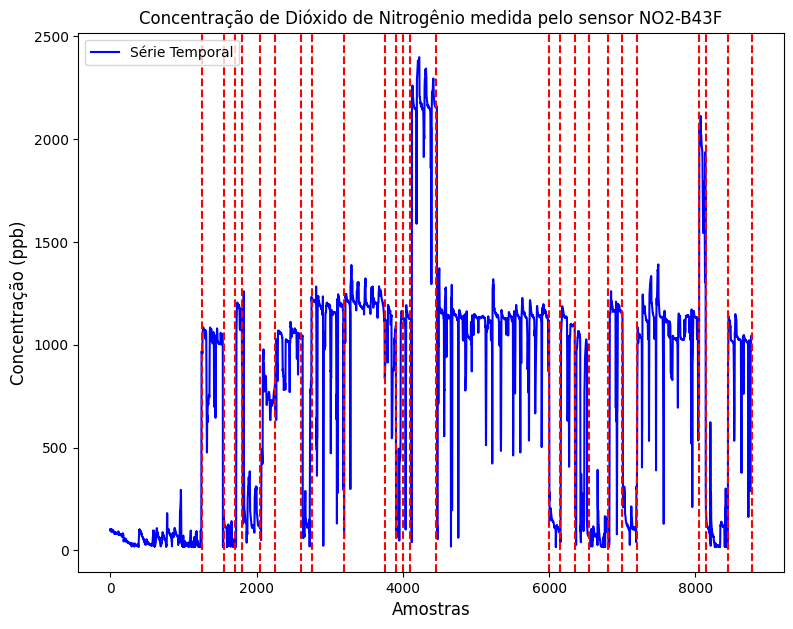
\includegraphics[width=\textwidth]{chapters/3-ANÁLISE DOS DADOS/Figuras/rebase-no2-b43f.png}
        \caption{Pontos de alteração da linha base detectados pelo algoritmo \acrshort{pelt}}
        \label{fig:data-rebase-no2}
    \end{subfigure}
    \hfill
    \label{fig:data-no2-raw-and-pelt}
\end{figure}

A Figura \ref{fig:data-no2-raw} mostra a série temporal do sensor depois de removidos os valores fora de intervalo. Observa-se que a partir do final do mês de dezembro ocorreram seguidas alterações de linha base, detectadas pelo algoritmo \acrshort{pelt}, conforme se ilustra na Figura \ref{fig:data-rebase-no2}. Dado que as mudanças de linha base se mantiveram de forma continuada a partir desse mês, para o restante das análises apenas foram consideradas as leituras anteriores à primeira alteração da linha base do sensor. A Figura \ref{fig:data-no2-preproc-hist} mostra o histograma dos dados das leituras prévias às alterações de linha base, os quais apresentaram uma distribuição log-normal. A Figura \ref{fig:data-co-preproc-1HR} mostra a série temporal das leituras do sensor NO2-B43F após aplicar a metodologia de pré-processamento e re-amostrar os dados para um período de 1 hora.

\begin{figure}[h]
    \centering
    \caption{Histograma das leituras do sensor NO2-B43F}
    \begin{subfigure}{0.4\textwidth}
        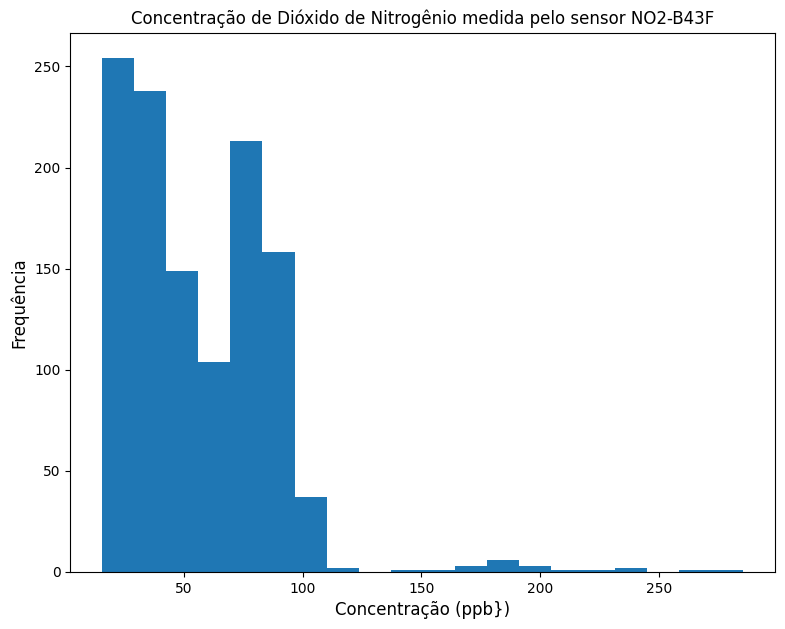
\includegraphics[width=\textwidth]{chapters/3-ANÁLISE DOS DADOS/Figuras/preproc-hist-no2-B43F.png}
        \caption{Histograma após à remoção das alterações de linha base}
        \label{fig:data-no2-preproc-hist}
    \end{subfigure}
    \hfill
    \begin{subfigure}{0.4\textwidth}
        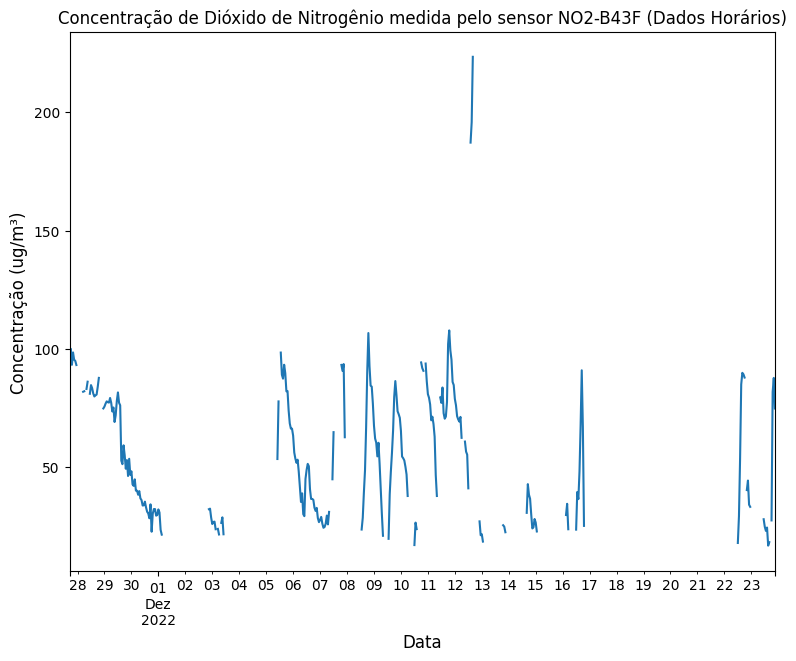
\includegraphics[width=\textwidth]{chapters/3-ANÁLISE DOS DADOS/Figuras/preproc-1HR-no2-B43F.png}
        \caption{Série temporal pré-processada do sensor NO2-B43F com T = 1 hr}
        \label{fig:data-co-preproc-1HR}
    \end{subfigure}
    \label{fig:data-no2-preproc}
\end{figure}

A Figura \ref{fig:data-no2-preproc-box} mostra a série de dados pré-processados do sensor NO2-B43F, juntamente com um gráfico de caixas que representa o comportamento diário das leituras agrupadas por hora do dia. Neste último não é possível perceber um padrão de comportamento muito claro nos dados ao longo do dia, mas em geral observa-se que foram registradas valores de concentração mais altos entre as 14 - 19 hrs. Na Figura \ref{fig:data-no2-reference-box} apresenta-se a série temporal da concentração de referência e seu comportamento diário ao longo do mesmo período. Nas leituras de referência também não é possível observar um padrão diário nos dados.

\begin{figure}[h]
    \centering
    \begin{subfigure}{0.9\textwidth}
        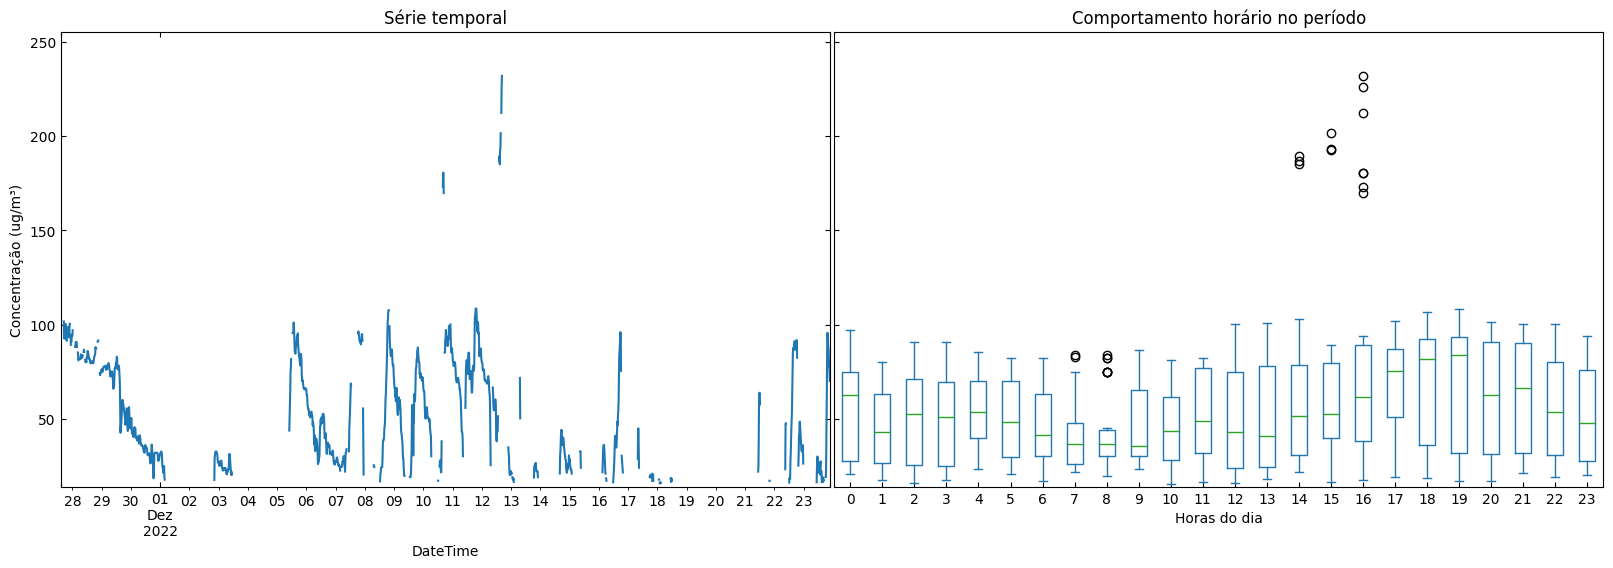
\includegraphics[width=\textwidth]{chapters/3-ANÁLISE DOS DADOS/Figuras/preproc-no2-B43F.png}
        \caption{Série temporal do sensor pré-processada (T = 15 mins) e seu comportamento diário}
        \label{fig:data-no2-preproc-box}
    \end{subfigure}
    \hfill
    \centering
    \begin{subfigure}{0.9\textwidth}
        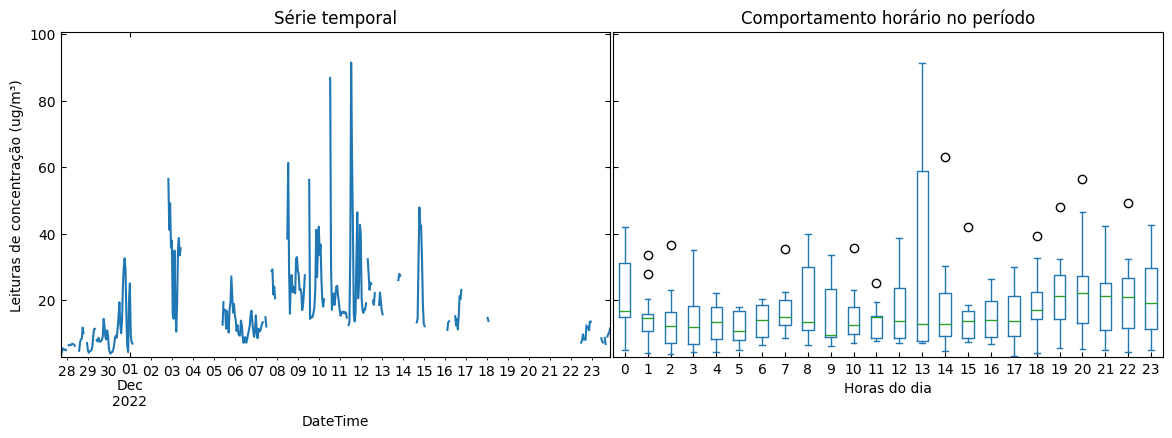
\includegraphics[width=\textwidth]{chapters/3-ANÁLISE DOS DADOS/Figuras/no2-reference-series-and-box.png}
        \caption{Série temporal das leituras de concentração de referência (T = 1 H) e seu comportamento diário}
        \label{fig:data-no2-reference-box}
    \end{subfigure}
    \hfill
    \label{fig:data-no2-box}
\end{figure}

A Tabela \ref{tab:data-contab-no2} mostra a contagem dos dados etiquetados para períodos de 15 minutos e de 1 hora. Observa-se que dos 17647 pontos de dados, que representavam as amostras adquiridas com um período de 15 minutos no intervalo de 20/11/2022 até 23/05/2023, 1175 foram aproveitados como dados válidos, o que representa um 7 \% aproximadamente dos dados originais. Ao re-amostrar esses 1175 pontos em dados horários obtiveram-se 285 amostras horárias de concentração válidas (aproximadamente 45 \% dos dados) para realizar a calibração.

\begin{table}[h]
    \caption{Contabilização das leituras do sensor CO-B4 por etiquetas}
    \centering
    \begin{tabularx}{0.95\textwidth}[h]{
         >{\raggedright\hsize=.475\hsize\arraybackslash}X
         >{\raggedright\hsize=.20\hsize\arraybackslash}X 
         >{\raggedright\hsize=.5\hsize\arraybackslash}X
        | >{\raggedright\hsize=.50\hsize\arraybackslash}X 
         >{\raggedright\hsize=.20\hsize\arraybackslash}X 
         >{\raggedright\hsize=.5\hsize\arraybackslash}X }
        \multicolumn{3}{c|}{Série temporal T = 15 mins} & \multicolumn{3}{c}{Série temporal T = 1 hr} \\
        \hline
        Etiquetas & No. amostras & \% amostras & Etiquetas & No. amostras & \% amostras \\ [0.5ex]
        \hline
        \textit{MISSING} & 5767 & 32.68 \% & \textit{LOWSAMPLES} & 347 & 54.91 \% \\ [0.5ex]
        
        \textit{LTLL} & 2438 & 13.82 \% & \textit{VALID} & 285 & 45.09 \% \\ [0.5ex]
        
        \textit{GTUL} & 0.0 & 0.0 \% & & & \\ [0.5ex]
        
        \textit{STABILIZING} & 673 & 3.81 \% & & & \\ [0.5ex]
        
        \textit{BADSPIKE} & 1 & 0.01 \% & & & \\ [0.5ex]
        
        \textit{LTQTLE01} & 32 & 0.18 \% & & & \\ [0.5ex]
        
        \textit{GTQTLE99} & 36 & 0.20 \% & & & \\ [0.5ex]
        
        \textit{REBASE} & 7525 & 42.64 \% & & & \\ [0.5ex]
        
        \textit{VALID} & 1175 & 6.66 \% & & & \\ [0.5ex]
        \hline
        TOTAL & 17647 & & TOTAL & 632 & \\
    \end{tabularx}
    \label{tab:data-contab-no2}
\end{table}

\subsection{Dependência com a temperatura}

Investigou-se a existência de correlação entre as leituras do sensor de \acrshort{no2} e as variações de temperatura medida no interior da câmara de medição. Para tal, foram empregados os testes estatísticos de correlação de Spearman e Kendall. Os resultados desses testes revelaram coeficientes de correlação baixos. O coeficiente de Spearman calculado foi de 0.09, com um valor de p inferior a 0.5. De maneira semelhante, o coeficiente de Kendall foi de 0.06, também com p < 0.05. Ao avaliar a hipótese nula de ausência de correlação, os resultados forneceram evidências robustas para sua rejeição, sugerindo que existe correlação, embora baixa, entre as leituras do sensor de \acrshort{no2} e as variações de temperatura. A Figura \ref{fig:data-temp-no2-corr} mostra um gráfico de dispersão entre os dados do sensor e a temperatura, ilustrando os resultados de correlação obtidos. As leituras de referência mostraram um comportamento diferente, não apresentando correlação com a variável temperatura. Os testes estatísticos de Spearman e Kendall mostraram que não foi possível rejeitar a hipótese nula de não existência de correlação entre as variáveis (Figura \ref{fig:data-temp-no2-ref-corr}).

\begin{figure}[h]
    \centering
    \caption{Relação dos dados de concentração de \acrshort{no2} com a temperatura}
    \begin{subfigure}{0.4\textwidth}
        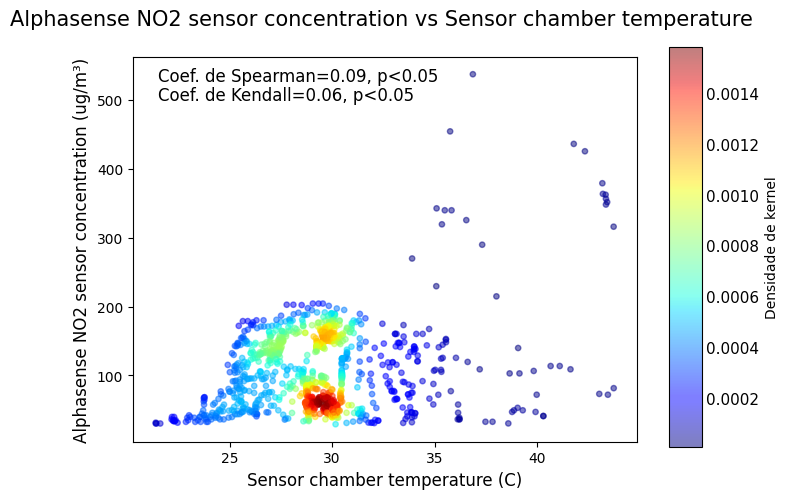
\includegraphics[width=\textwidth]{chapters/3-ANÁLISE DOS DADOS/Figuras/temperature-no2-B43F.png}
        \caption{Relação entre as leituras do sensor NO2-B43F (\(\mu g/m^3\)) e a temperatura (\textdegree C)}
        \label{fig:data-temp-no2-corr}
    \end{subfigure}
    \hfill
    \begin{subfigure}{0.4\textwidth}
        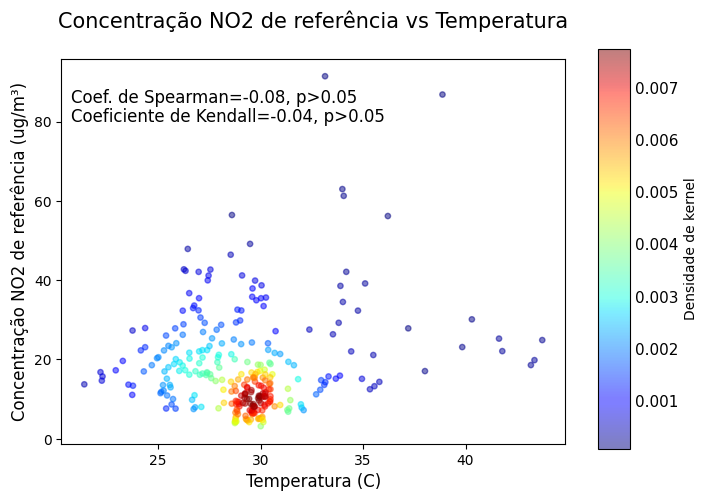
\includegraphics[width=\textwidth]{chapters/3-ANÁLISE DOS DADOS/Figuras/temperature-no2-reference.png}
        \caption{Relação entre os valores de concentração de referência (\(\mu g/m^3\)) e a temperatura (\textdegree C)}
        \label{fig:data-temp-no2-ref-corr}
    \end{subfigure}
    \hfill
    \label{fig:data-no2-temp}
\end{figure}

\subsection{Comparação das leituras de \acrshort{no2} do sensor NO2-B43F com as medições de referência}

Nas Figuras \ref{fig:data-no2-reference-time-series} e \ref{fig:data-no2-reference-corr} apresentam-se as leituras de \acrshort{no2} obtidas pelo sensor NO2-B43F de Alphasense e a estação de referência. Observa-se que as leituras do sensor superestimaram os valores de concentração de referência com valores aproximadamente 5 vezes maiores. Os testes de Spearman e Kendall revelaram que não foi possível rejeitar a hipótese nula de que não existe correlação entre os dados do sensor e da estação de referência.

\begin{figure}[h!]
    \centering
    \caption{Séries temporais e gráficos de dispersão das medições de \acrshort{no2}}
    \begin{subfigure}{0.44\textwidth}
        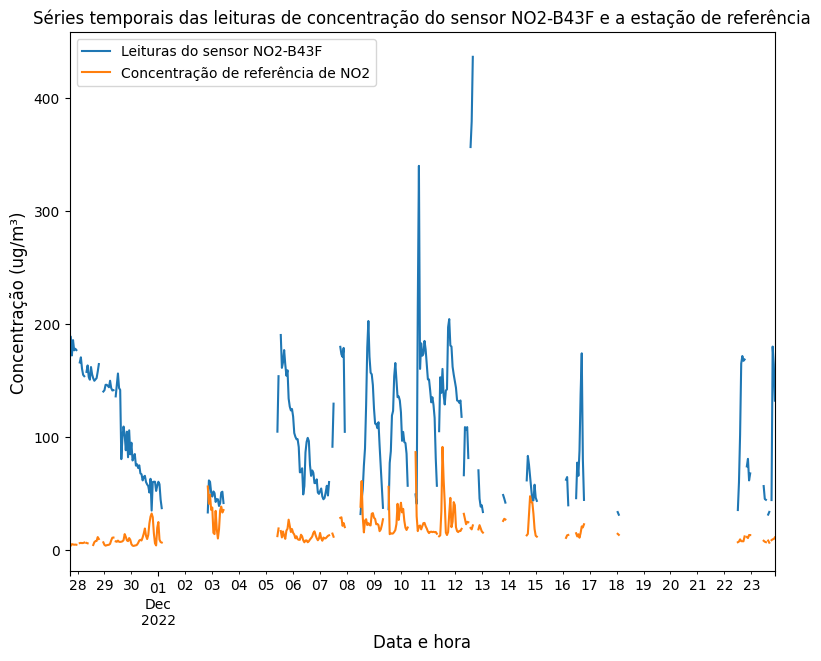
\includegraphics[width=\textwidth]{chapters/3-ANÁLISE DOS DADOS/Figuras/no2-b43F-reference-time-series.png}
        \caption{Séries temporais das leituras de \acrshort{no2} do sensor NO2-B43F e a estação de referência}
        \label{fig:data-no2-reference-time-series}
    \end{subfigure}
    \hfill
    \begin{subfigure}{0.54\textwidth}
        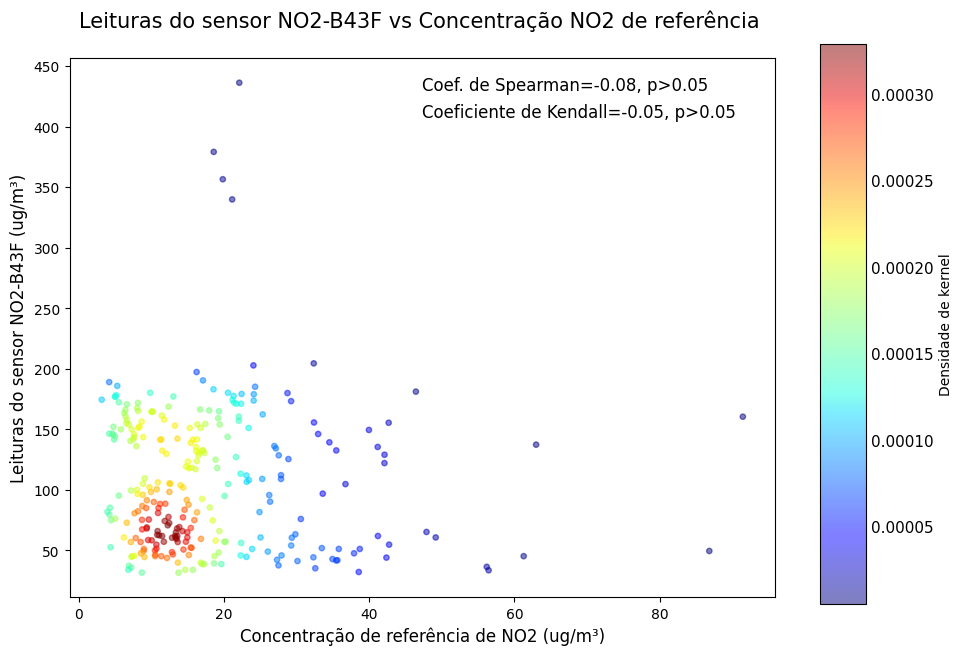
\includegraphics[width=\textwidth]{chapters/3-ANÁLISE DOS DADOS/Figuras/no2-b43F-reference-correlation.png}
        \caption{Gráfico de dispersão das leituras de \acrshort{no2} do sensor NO2-B43F e a estação de referência}
        \label{fig:data-no2-reference-corr}
    \end{subfigure}
\end{figure}


\subsection{Preprocessamento dos dados de Material Particulado (MP-10)}

A Figura \ref{fig:data-pm10-raw} mostra a série temporal do sensor de \acrshort{mp10} depois de removidos os valores fora de intervalo. Os resultados do pré-processamento das leituras do sensor são ilustrados nas Figuras \ref{fig:data-pm10-preproc-hist} e \ref{fig:data-pm10-preproc-15} que apresentam, respectivamente, o histograma dos dados e a série pré-processada do sensor OPC-N3 juntamente com o comportamento diário das medições ao longo do período sob análise agrupados por hora do dia. Os dados foram re-amostrados para um período de 1 hora para serem calibrados com as leituras de referência, a Figura \ref{fig:data-pm10-preproc-1HR} mostra a série temporal resultante da re-amostragem.

\begin{figure}[h]
    \centering
    \caption{Série temporal das leituras do sensor OPC-N3}
    \begin{subfigure}{0.495\textwidth}
        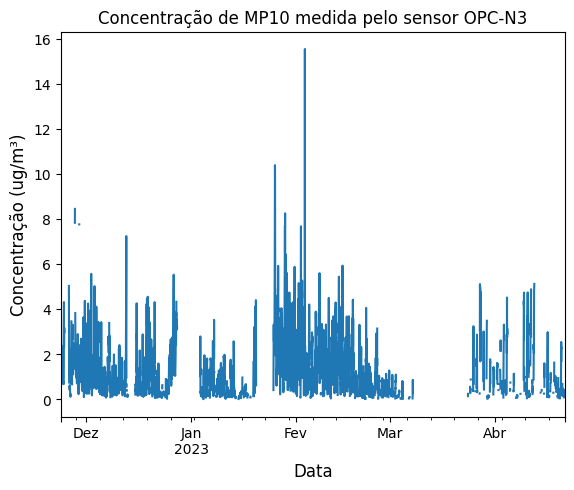
\includegraphics[width=\textwidth]{chapters/3-ANÁLISE DOS DADOS/Figuras/raw-pm10.png}
        \caption{Série temporal do sensor depois de remover valores fora de intervalo}
        \label{fig:data-pm10-raw}
    \end{subfigure}
    \hfill
    \begin{subfigure}{0.495\textwidth}
        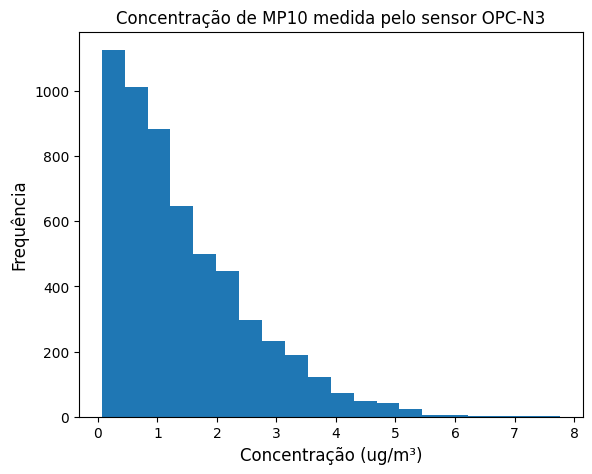
\includegraphics[width=\textwidth]{chapters/3-ANÁLISE DOS DADOS/Figuras/preproc-hist-pm10.png}
        \caption{Histograma das leituras pré-processadas do sensor OPC-N3}
        \label{fig:data-pm10-preproc-hist}
    \end{subfigure}
    \begin{subfigure}{0.99\textwidth}
        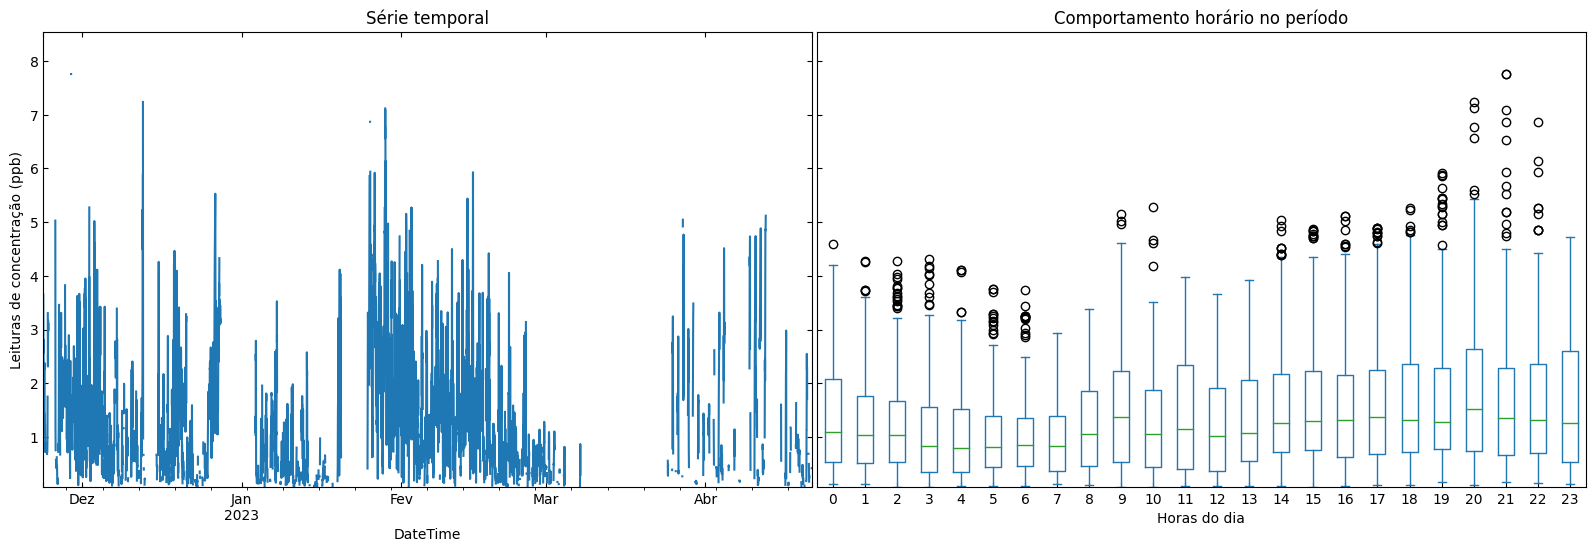
\includegraphics[width=\textwidth]{chapters/3-ANÁLISE DOS DADOS/Figuras/preproc-pm10.png}
        \caption{Série temporal do sensor pré-processada (T = 15 mins) e seu comportamento diário}
        \label{fig:data-pm10-preproc-15}
    \end{subfigure}
    \hfill
    \label{fig:data-pm10-15}
    \fonte{Desenvolvido pelo autor (2023)}
\end{figure}

\begin{figure}[h]
    \centering
    \caption{Série temporal horária das leituras do sensor OPC-N3 e sua relação com a temperatura}
    \begin{subfigure}{0.495\textwidth}
        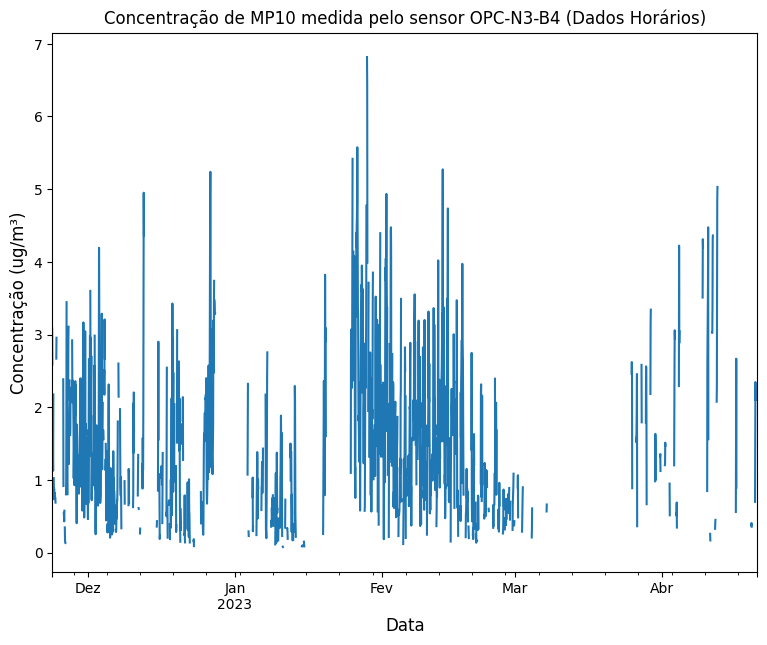
\includegraphics[width=\textwidth]{chapters/3-ANÁLISE DOS DADOS/Figuras/preproc-1HR-pm10.png}
        \caption{Série temporal com T = 1 hr}
        \label{fig:data-pm10-preproc-1HR}
    \end{subfigure}
    \hfill
    \begin{subfigure}{0.495\textwidth}
        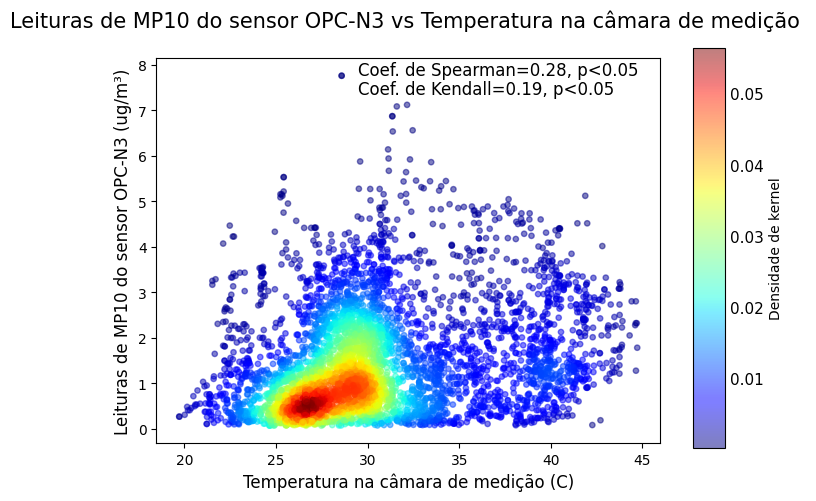
\includegraphics[width=\textwidth]{chapters/3-ANÁLISE DOS DADOS/Figuras/temperature-pm10.png}
        \caption{Relação entre as leituras do sensor OPC-N3 e a temperatura}
        \label{fig:data-temp-pm10-corr}
    \end{subfigure}
    \fonte{Desenvolvido pelo autor (2023)}
\end{figure}

Na Tabela \ref{tab:data-contab-pm10} contabilizam-se os dados para período de 15 minutos e de 1 hora. Observa-se que dos 14541 pontos de dados, que representavam as amostras adquiridas com um período de 15 minutos no intervalo de 21/11/2022 até 21/04/2023, 5668 foram aproveitados como dados válidos, o que representa um 39 \% aproximadamente dos dados originais. Ao re-amostrar esses 5668 pontos em dados horários obtiveram-se 1291 amostras horárias de concentração válidas (aproximadamente 36 \% dos dados) para realizar a calibração. Vale salientar que nos dados de \acrshort{mp10} não foram encontradas alterações na linha base nem dados de estabilização já que esse sensor não precisa desse intervalo prévio as medições.

\begin{table}[h]
    \caption{Contabilização dos dados por etiquetas das leituras do sensor OPC-N3}
    \centering
    \begin{tabularx}{0.95\textwidth}[h]{
         >{\raggedright\hsize=.45\hsize\arraybackslash}X
         >{\raggedright\hsize=.20\hsize\arraybackslash}X 
         >{\raggedright\hsize=.5\hsize\arraybackslash}X
         >{\raggedright\hsize=.50\hsize\arraybackslash}X 
         >{\raggedright\hsize=.20\hsize\arraybackslash}X 
         >{\raggedright\hsize=.5\hsize\arraybackslash}X }
        \multicolumn{3}{c}{Série temporal T = 15 mins} & \multicolumn{3}{c}{Série temporal T = 1 hr} \\
        \hline
        Etiquetas & No. amostras & \% amostras & Etiquetas & No. amostras & \% amostras \\ [0.5ex]
        \hline
        \textit{MISSING} & 6053 & 41.63 \% & \textit{LOWSAMPLES} & 2291 & 63.96 \% \\ [0.5ex]
        
        \textit{LTLL} & 1297 & 8.92 \% & \textit{VALID} & 1291 & 36.04 \% \\ [0.5ex]
        
        \textit{GTUL} & 0 & 0.0 \% & & & \\ [0.5ex]
        
        \textit{STABILIZING} & 0 & 0.0 \% & & & \\ [0.5ex]
        
        \textit{BADSPIKE} & 1332 & 9.16 \% & & & \\ [0.5ex]
        
        \textit{LTQTLE01} & 117 & 0.80 \% & & & \\ [0.5ex]
        
        \textit{GTQTLE99} & 74 & 0.51 \% & & & \\ [0.5ex]
        
        \textit{REBASE} & 0 & 0.0 \% & & & \\ [0.5ex]
        
        \textit{VALID} & 5668 & 38.98 \% & & & \\ [0.5ex]
        \hline
        TOTAL & 14541 & & TOTAL & 3582 & \\
    \end{tabularx}
    \label{tab:data-contab-pm10}
    \fonte{Desenvolvido pelo autor}
\end{table}

\subsubsection{Dependência com a temperatura}

Investigou-se a existência de correlação entre as leituras do sensor de \textit{mp10} e as variações de temperatura medida no interior da câmara de medição. Os resultados dos testes estatísticos de Spearman e Kendall revelaram coeficientes de correlação estatisticamente significativos, conforme se ilustra na Figura \ref{fig:data-temp-pm10-corr}. O coeficiente de Spearman resultou em 0.29 com um valor de p inferior a 0.05, indicando uma correlação estatisticamente significativa entre as leituras dos sensores e a temperatura. De maneira semelhante, o coeficiente de Kendall foi de 0.20, também com p < 0.05, reforçando a presença de uma associação significativa. Ao avaliar a hipótese nula de ausência de correlação, os resultados forneceram evidências para sua rejeição, sugerindo a existência de uma correlação entre as leituras dos sensores de \acrshort{mp10} e as variações de temperatura.

\section{Discussão}

Dos resultados descritos anteriormente observa-se que de modo geral a porcentagem das leituras que foram aproveitadas como válidas foi baixa, sendo os principais motivos a perda de dados (dados com leituras inválidas ou NaN) e as alterações de linha base. As leituras de \acrshort{mp10} apresentaram a maior porcentagem de dados válidos com aproximadamente 39 \% das leituras. Isso pode ter sido possível pelo fato do sensor OPC-N3 ter uma saída digital, produzindo maior estabilidade nas suas leituras. O sensor NO2-B43F teve a menor porcentagem com menos de 7 \% de dados válidos. Quase 43 \% das suas leituras sofreram alterações na linha base que impossibilitaram seu aproveitamento, o restante foram dados perdidos ou no período de estabilização. Dentre os sensores eletroquímicos utilizados, os que melhor desempenharam em termos de quantidade de leituras aproveitáveis foram os dois sensores OX-B431, que tiveram 30 e 74 \% de leituras válidas aproximadamente.

Os dados perdidos estão associados a falhas no equipamento como quedas de energia, falhas na leitura dos sensores que produziram valores NaN, erros de escrita no cartão de memória e erros na obtenção de carimbos de data e hora para os dados. Por outro lado, o motivo das alterações frequentes de linha base não foi possível descobrir a partir das informações com que se conta até o momento. O fato das alterações ocorrerem em momentos distintos para cada sensor faz pensar que não foram produzidas por falhas generalizadas na operação do equipamento, e sim com o funcionamento de sensores particulares.

Uma vez identificados os dados válidos comprovou-se que todos apresentaram distribuições log-normais, conforme o esperado para dados de concentração. Os sensores CO-B4 e OX-B431 (2) mostraram uma pequena bimodalidade ocasionada por uma possível dependência com a temperatura, já que foi identificado um perfil sazonal ao longo do dia coincidente com o perfil de temperatura diário. Em geral, com a exceção do sensor NO2-B43F, observou-se certa correlação entre as leituras dos sensores e a temperatura, principalmente nos dados de \acrshort{o3}. Esse comportamento era esperado dada a influência da radiação na concentração de \acrshort{o3} no ambiente, e pôde ser corroborado na análise das concentrações de referência. O sensor CO-B4 também gerou leituras correlacionadas com a temperatura, que não coincidiu com o comportamento dos dados de referência. A correlação das medições de referência foi baixa ($\rho$ = 0.18) em comparação com o sensor de baixo custo ($\rho$ = 0.52). É possível que essa suposta relação com a temperatura, inclusive no sensor de referência, tenha estado associada com padrões diários de poluição, sendo que a maior atividade antropogênica acontece na luz do dia, onde as temperaturas são mais elevadas. Contudo, o coeficiente de correlação mais elevado no sensor de baixo custo pode ser indício de uma certa influência com a temperatura, conforme já tem sido reportado na literatura. Nas leituras de \acrshort{no2} e \acrshort{mp10} a relação com a temperatura foi pouco perceptível.

De modo geral, a exceção dos sensores de \acrshort{o3}, o restante das leituras dos sensores de baixo custo apresentaram baixa correlação com as medições de referência, e diferenças elevadas na escala das medições. A maior correlação dos dados de ozônio pode explicar-se pelo próprio comportamento diário da variável que foi registrado pelos sensores, mas observou-se que o sensor OX-B431 (1) superestimou em quase 3 vezes as leituras originais, já o sensor 2 mostrou valores mais coerentes. A mesma diferença na ordem dos dados foi observada nas leituras do sensor NO2-B43F, com variações na escala de aproximadamente 4 vezes em relação com os dados originais.